\documentclass[12pt]{article} %tipo de documento

\usepackage[utf8]{inputenc}
\usepackage[spanish]{babel}
\usepackage{graphicx}
 \usepackage[section]{placeins}
\usepackage{fancyhdr}
\usepackage{hyperref}


\hypersetup{
    colorlinks=true,
    linkcolor=cyan,
    filecolor=magenta,      
    urlcolor=blue,
    }

\title{Void Rider\\\emph{Documento de Requerimientos}}
\author{Kenny Álvarez del Castillo Nava \and Karina Vellenaweth Moreno}



\begin{document}
 \renewcommand{\familydefault}{\sfdefault}
\pagestyle{fancy}


\maketitle

\newpage

\tableofcontents

\newpage

\section{Descripción}\label{descripcion}
\par Void Rider es un juego VR tipo arcade donde el jugador podra controlar el Void Rider, una nave espacial de combate, cuya misión es derrotar oleadas de enemigos que ponen en peligro la paz en la galaxia, la principal función que cubrira sera la de entrener al usuario

\section{Requerimientos funcionales}\label{funcionales}
\begin{itemize}
  \item Interacción con botones sin ayuda de los controles de el oculus
  \item Interacción con sliders sin ayuda de los controles de el oculus
  \item  Interacción de la nave con obstaculos
  \item  Interacción de la nave con enemigos
  \item  Solo un escenario presente en el juego
  \item  No hay interacción con powerups
  \item Pausa para el juego.

\end{itemize}

\section{Requerimientos no funcionales}\label{no funcionales}
\begin{itemize}
  \item Invertir el eje Y dentro del juego
  \item Opcion de juego multijugador
  \item Configuracion del audio
 \item Oculus Quest 2
 \item Blender
 \item Visual Code o Rider
 \item Unity version 2021.3.15f1
 \item Usuario estático al utilizar el juego
\item  Sin controles de Oculus Quest 2 (hand-tracking)
\end{itemize}


\section{Diagramas}\label{diagramas}
\subsection{Diagrama de Casos}

\begin{figure} [!htb]
  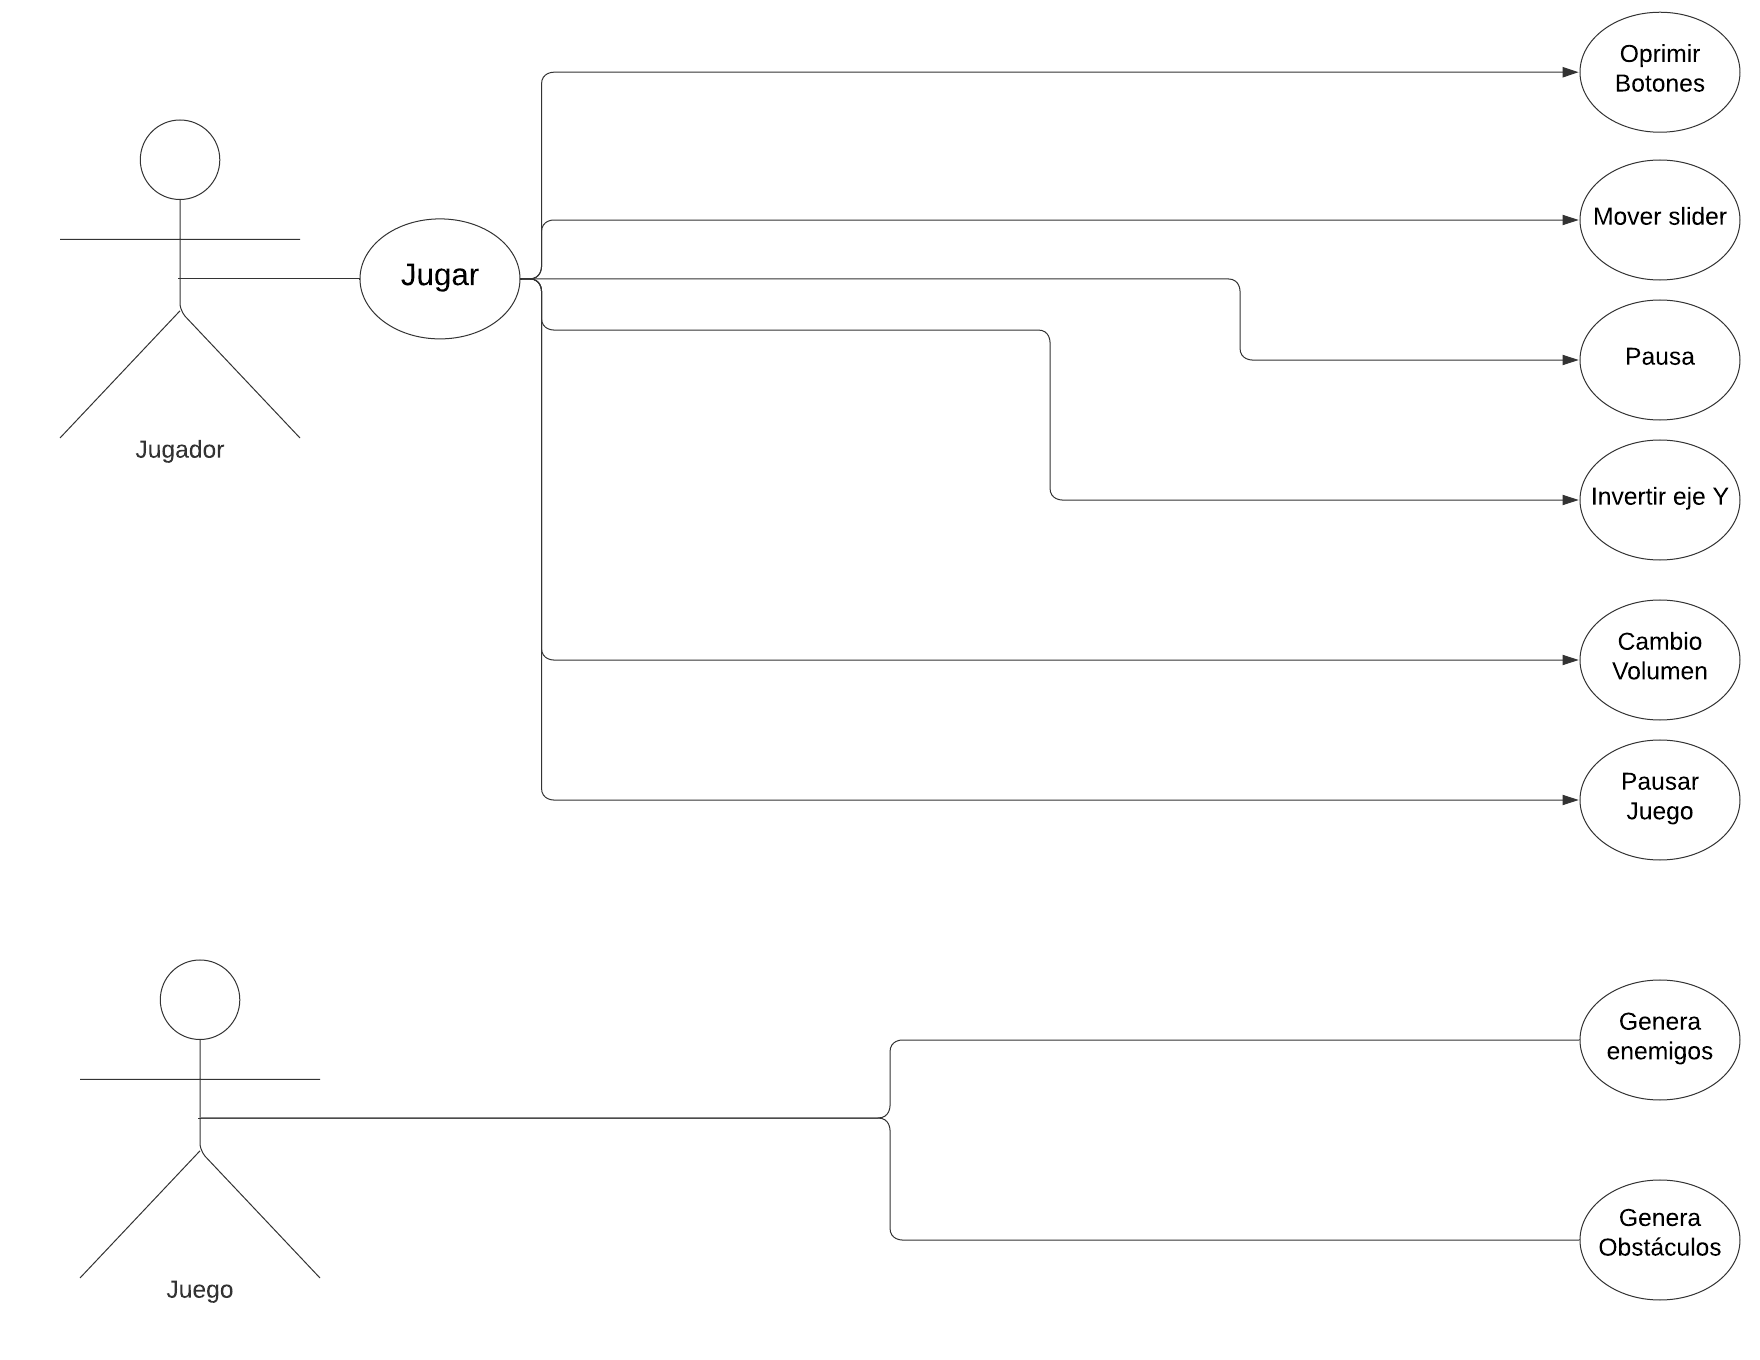
\includegraphics[width=\linewidth]{DiaCasos.png}
  \caption{Diagrama de casos}
  \label{fig:Diagrama1}
\end{figure}
\FloatBarrier
\newpage

\subsection{Diagrama de clases}
\begin{figure}  [!htb]
  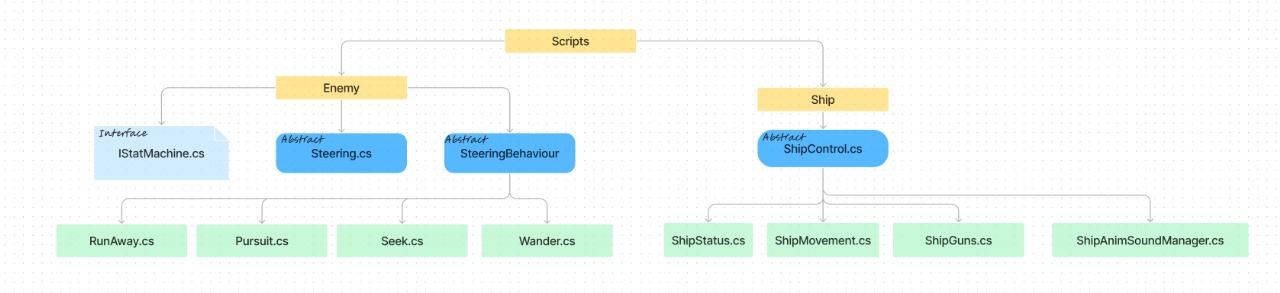
\includegraphics[width=\linewidth]{clases.jpg}
  \caption{Diagrama de clases}
  \label{fig:Diagrama1}
\end{figure}
\FloatBarrier
\newpage


\subsection{Diagramas de Secuencia}
\begin{figure}  [!htb]
  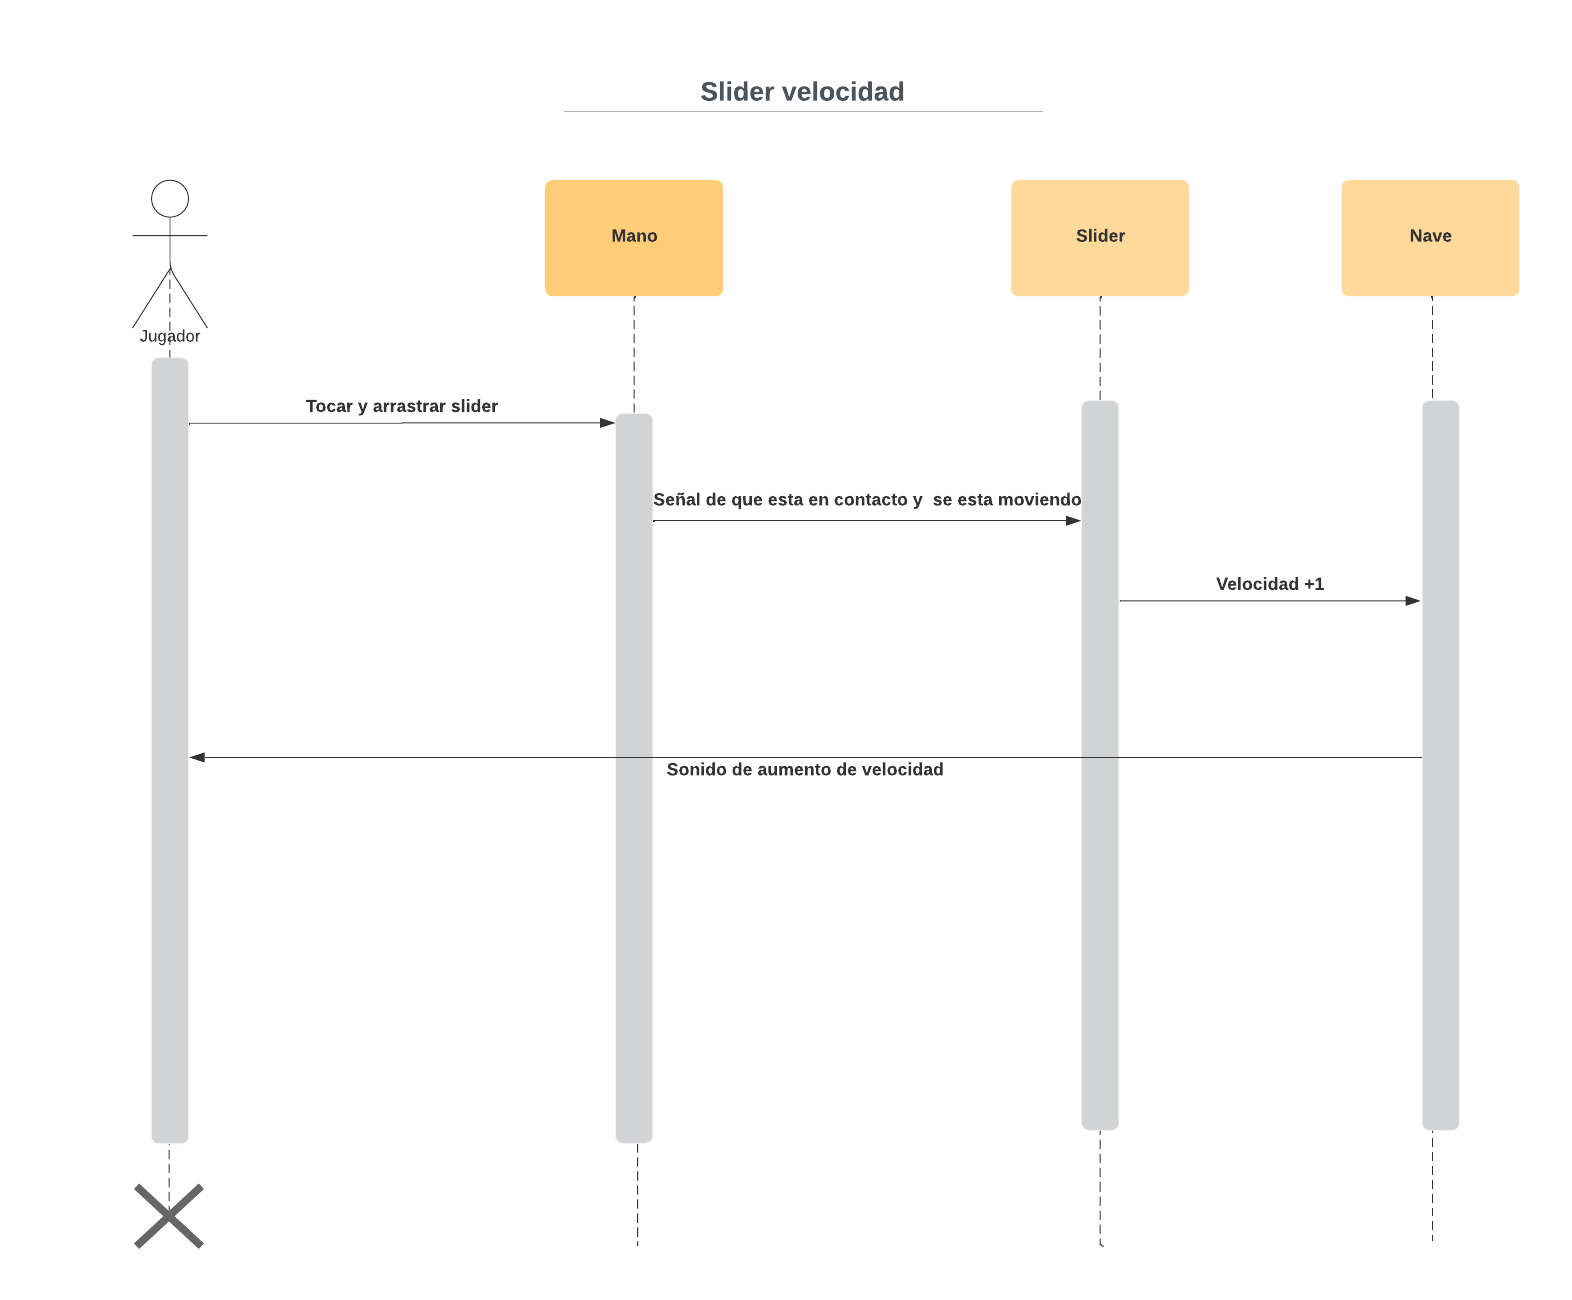
\includegraphics[width=\linewidth]{Diagrama secuencia slider.png}
  \caption{Diagrama secuencia slider velocidad}
\end{figure}

\begin{figure}  [!htb]
  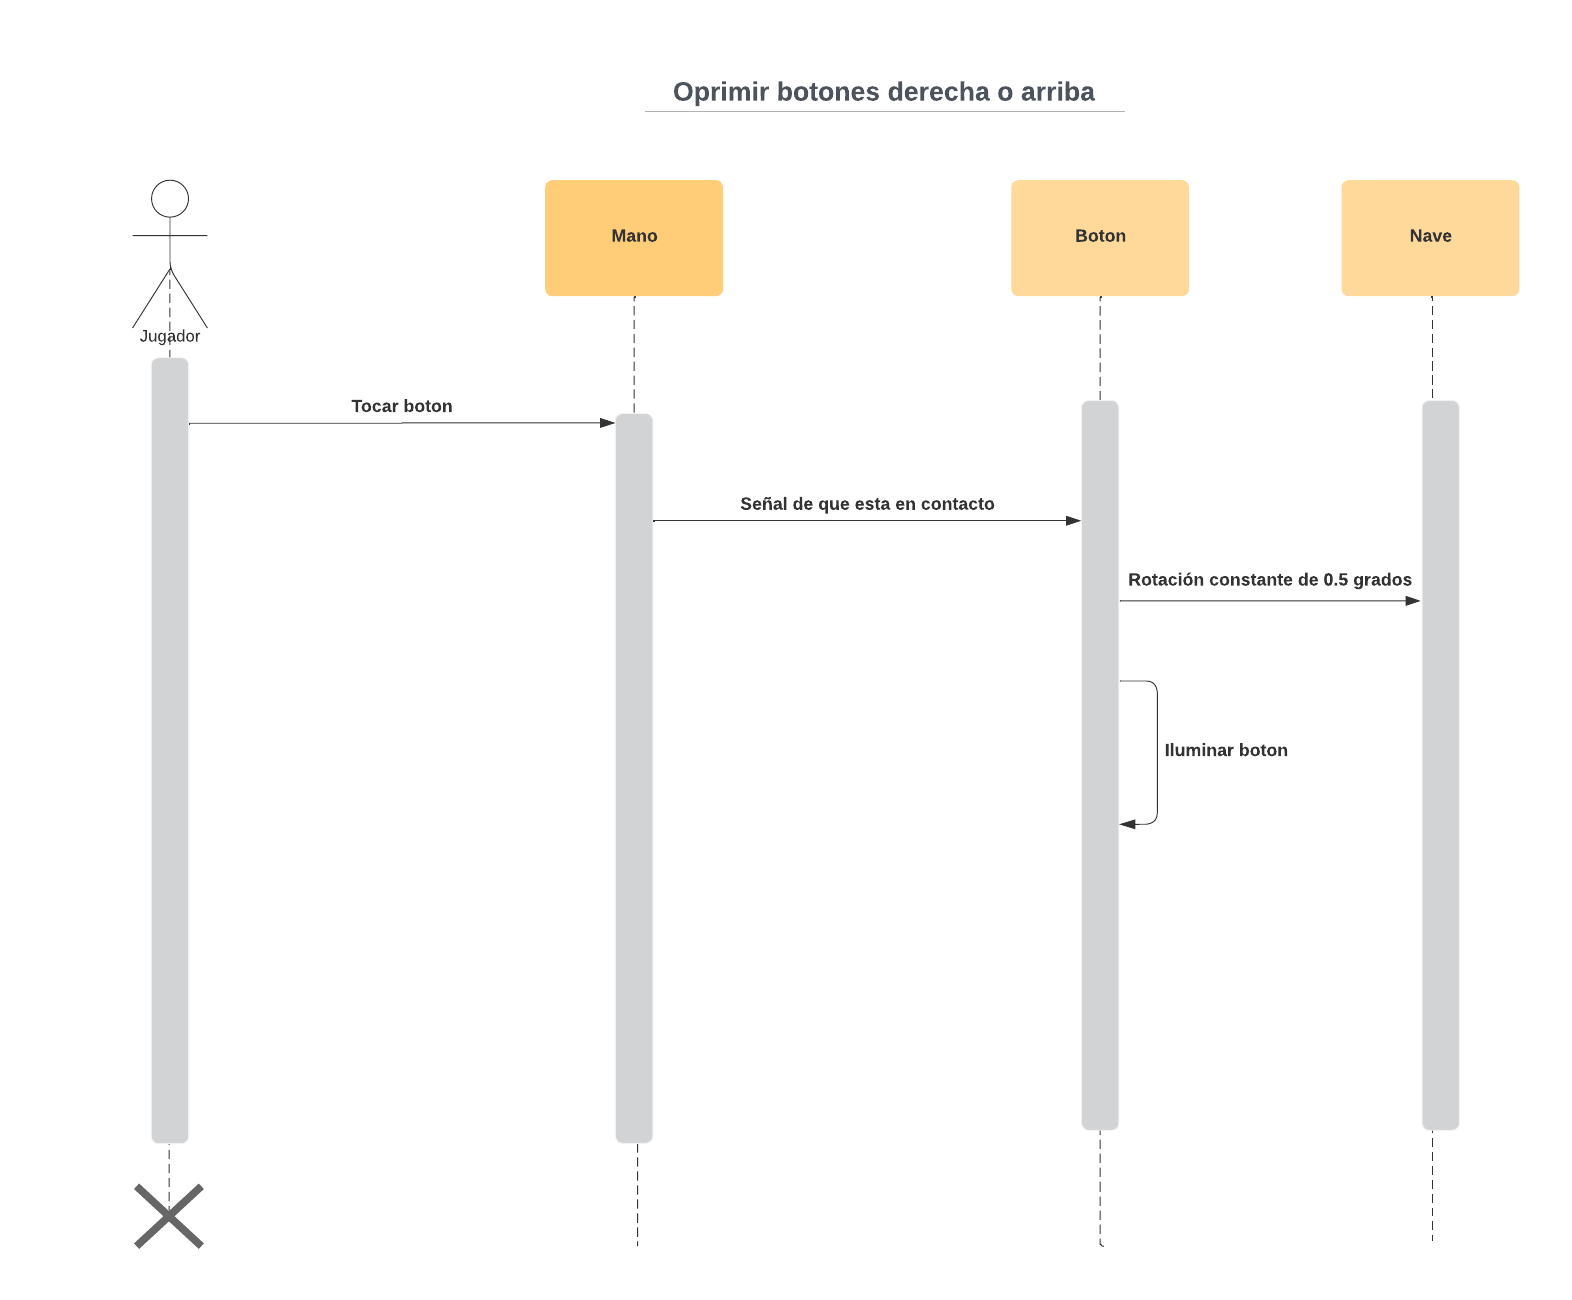
\includegraphics[width=\linewidth]{Diagrama secuencia oprimir botones 1.png}
  \caption{Diagrama secuencia botones direccion positiva}
\end{figure}

\begin{figure}  [!htb]
  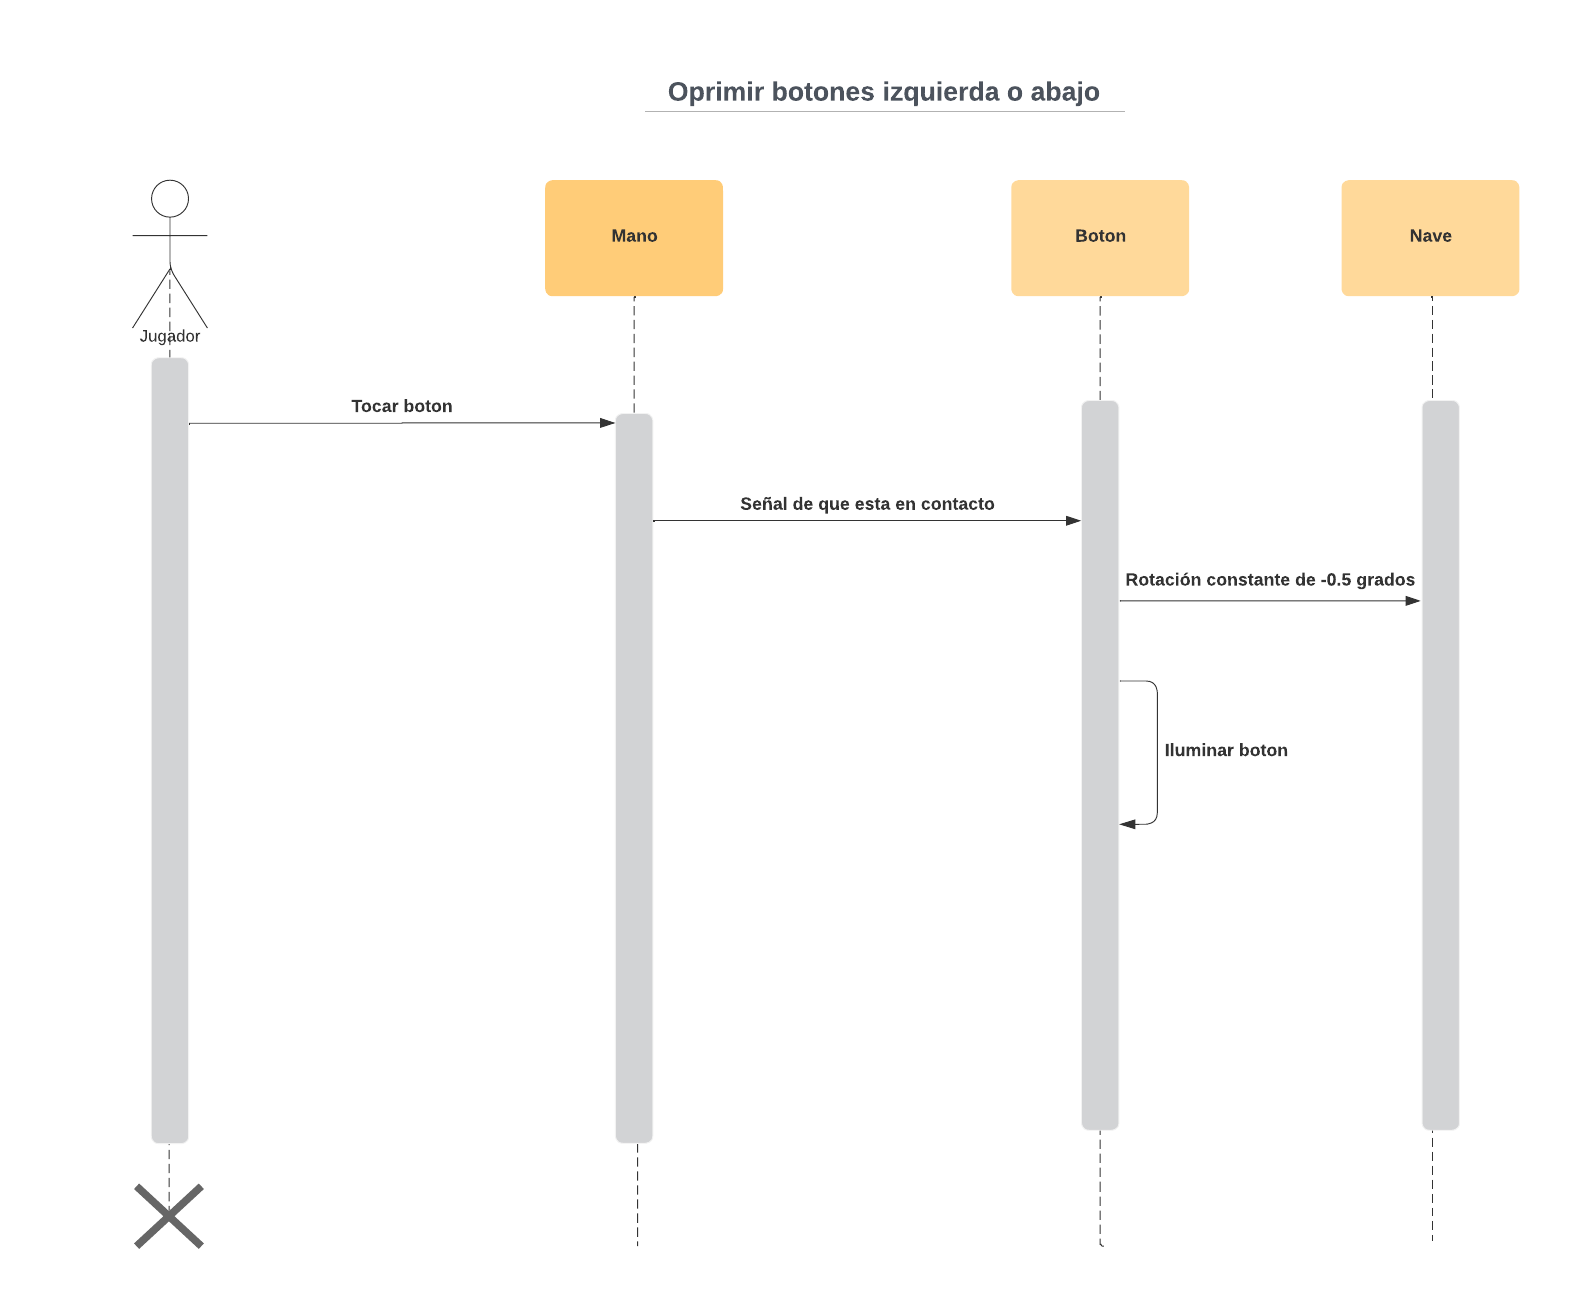
\includegraphics[width=\linewidth]{Diagrama secuencia oprimir botones 2.png}
  \caption{Diagrama secuencia botones direccion negativa}
\end{figure}

\begin{figure}  [!htb]
  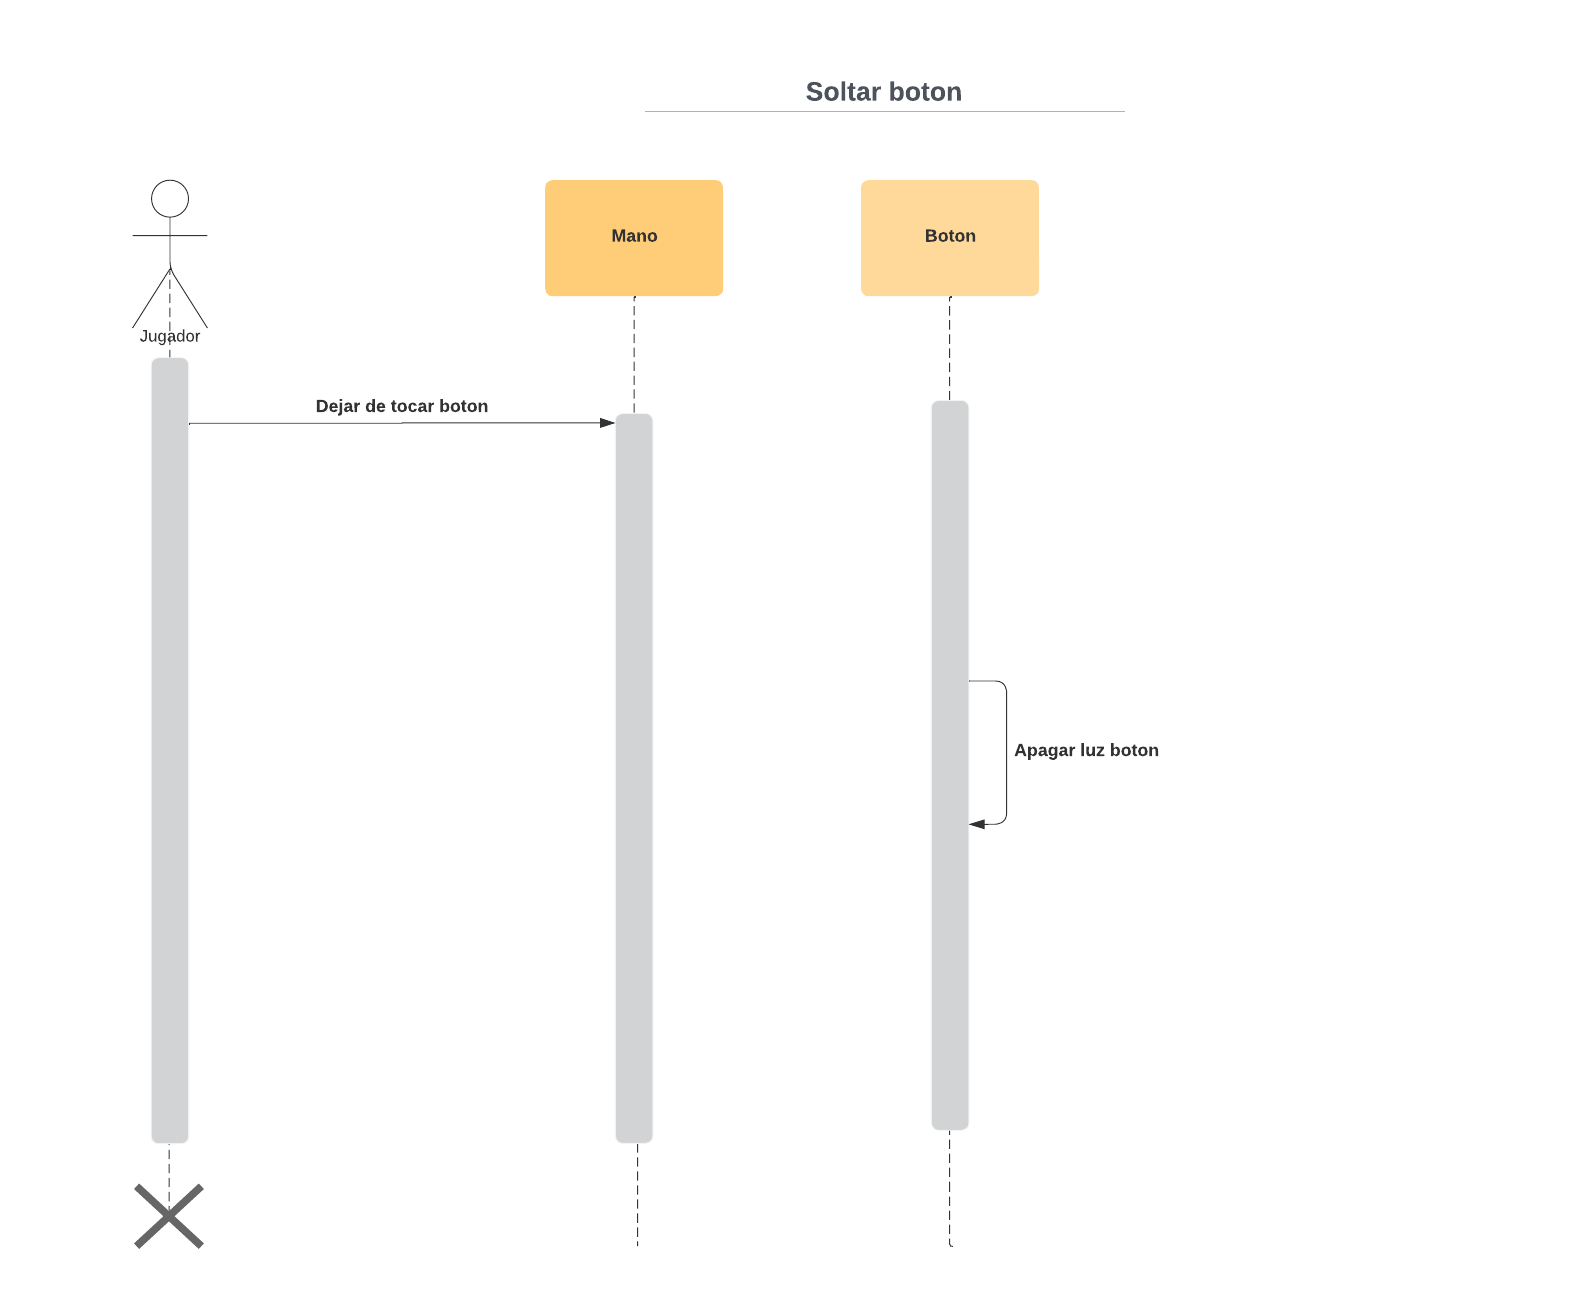
\includegraphics[width=\linewidth]{Diagrama secuencia soltar boton.png}
  \caption{Diagrama secuencia soltar botones}
\end{figure}

\begin{figure}  [!htb]
  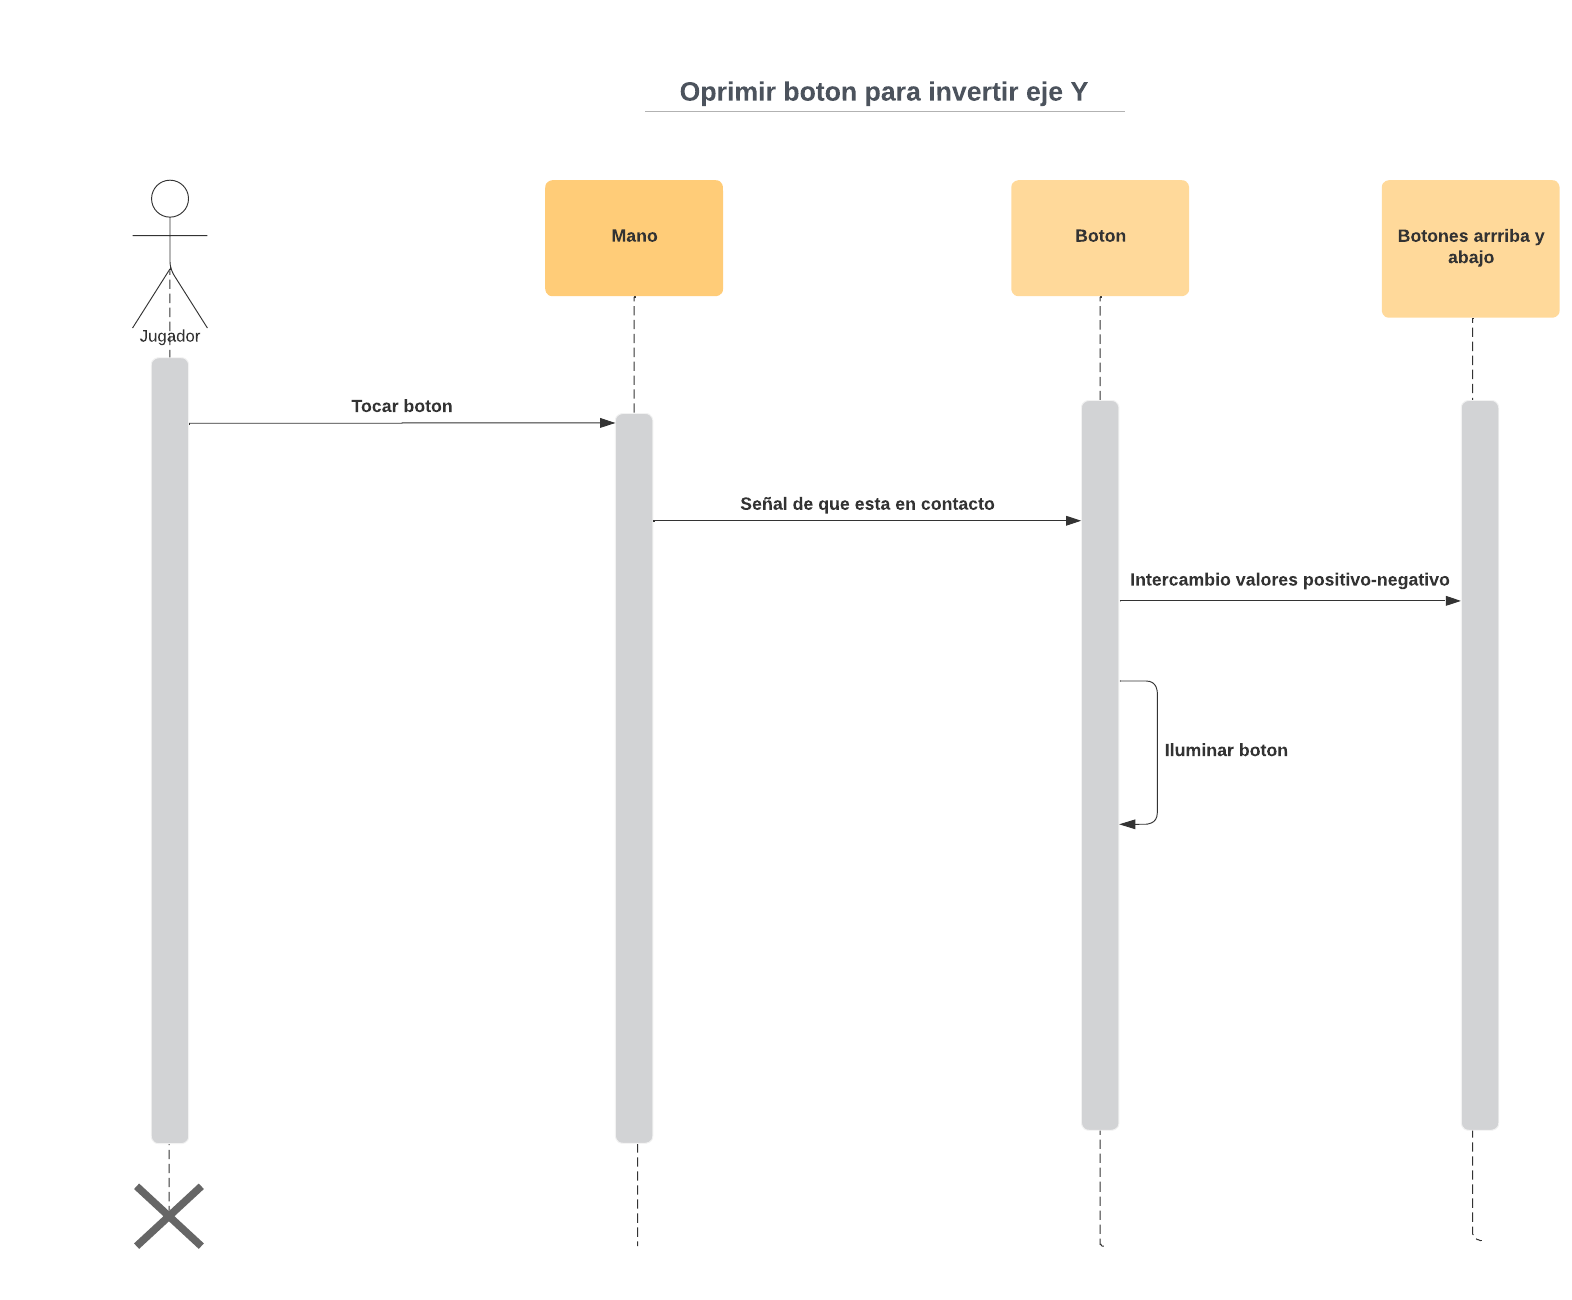
\includegraphics[width=\linewidth]{Diagrama secuencia oprimir boton eje y.png}
  \caption{Diagrama secuencia botones cambio eje}
\end{figure}

\begin{figure}  [!htb]
  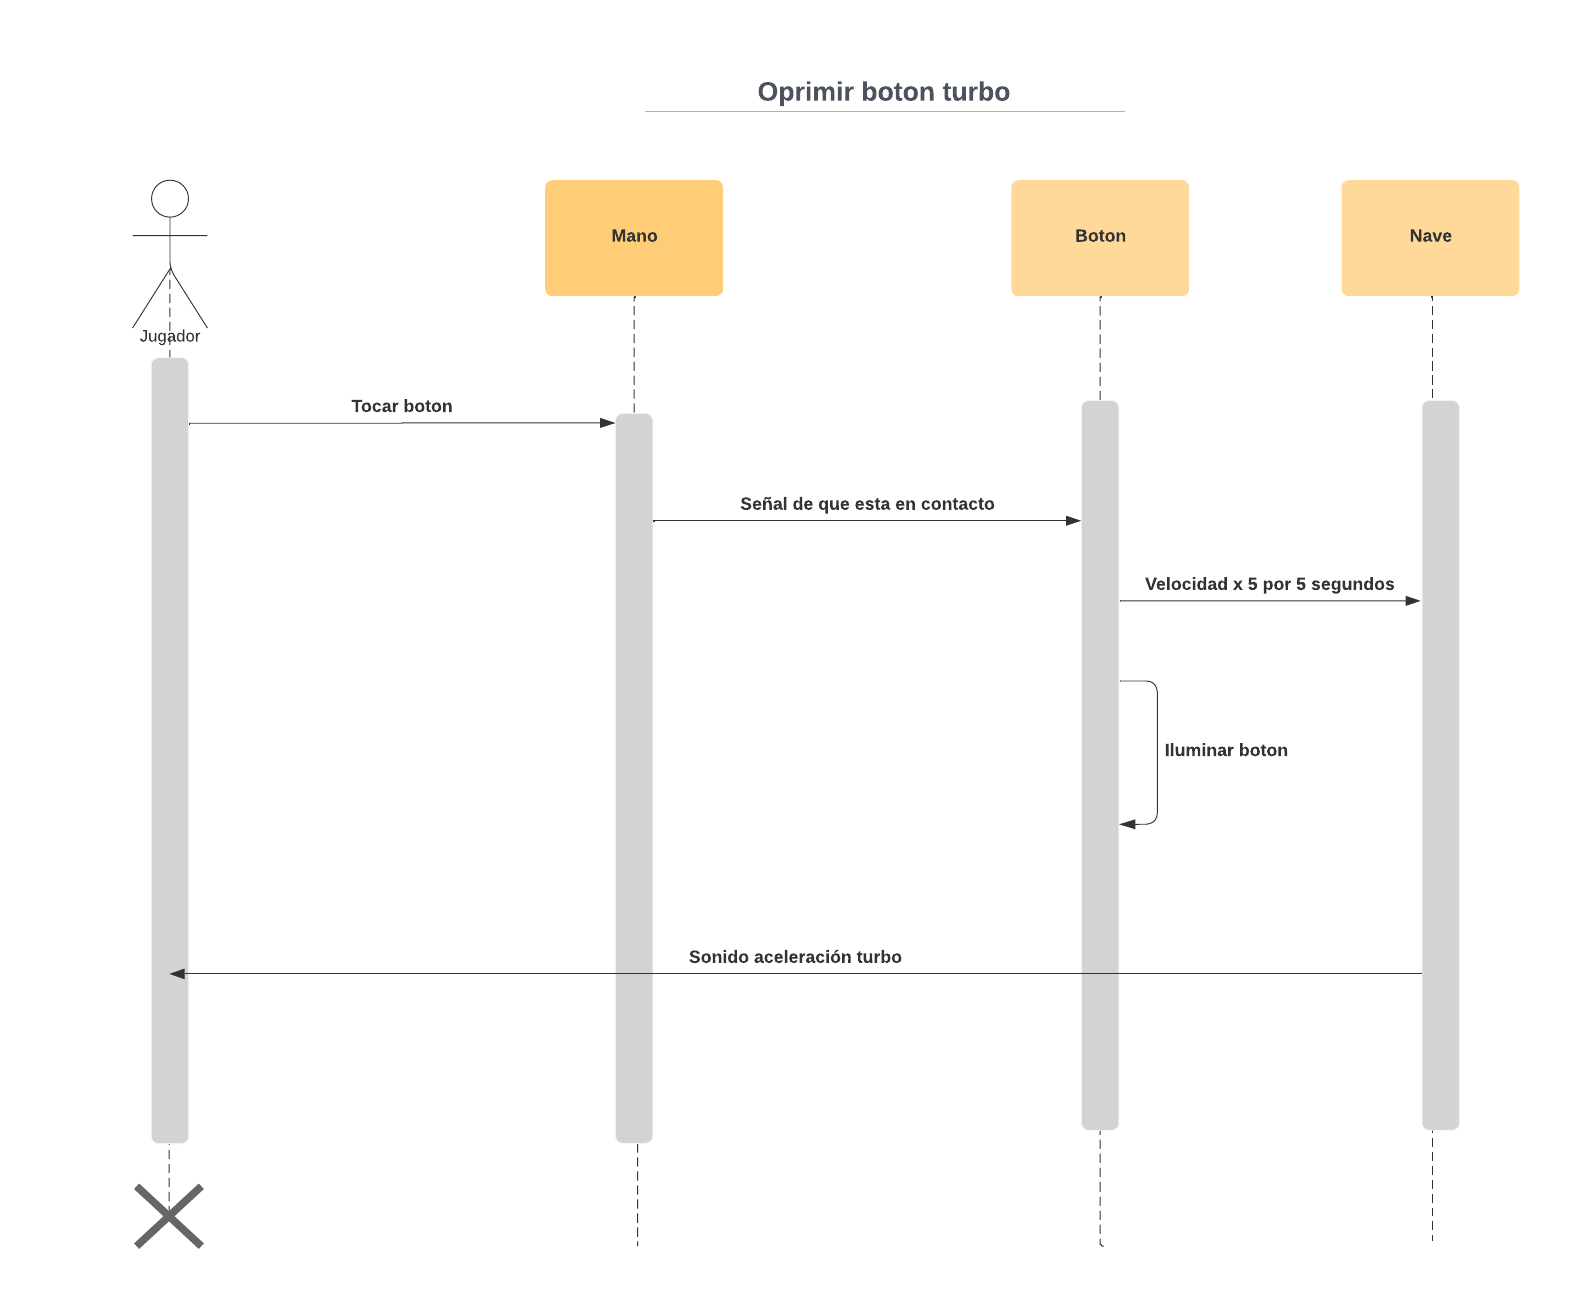
\includegraphics[width=\linewidth]{Diagrama secuencia oprimir boton turbo.png}
  \caption{Diagrama secuencia botones turbo}
\end{figure}

\begin{figure}  [!htb]
  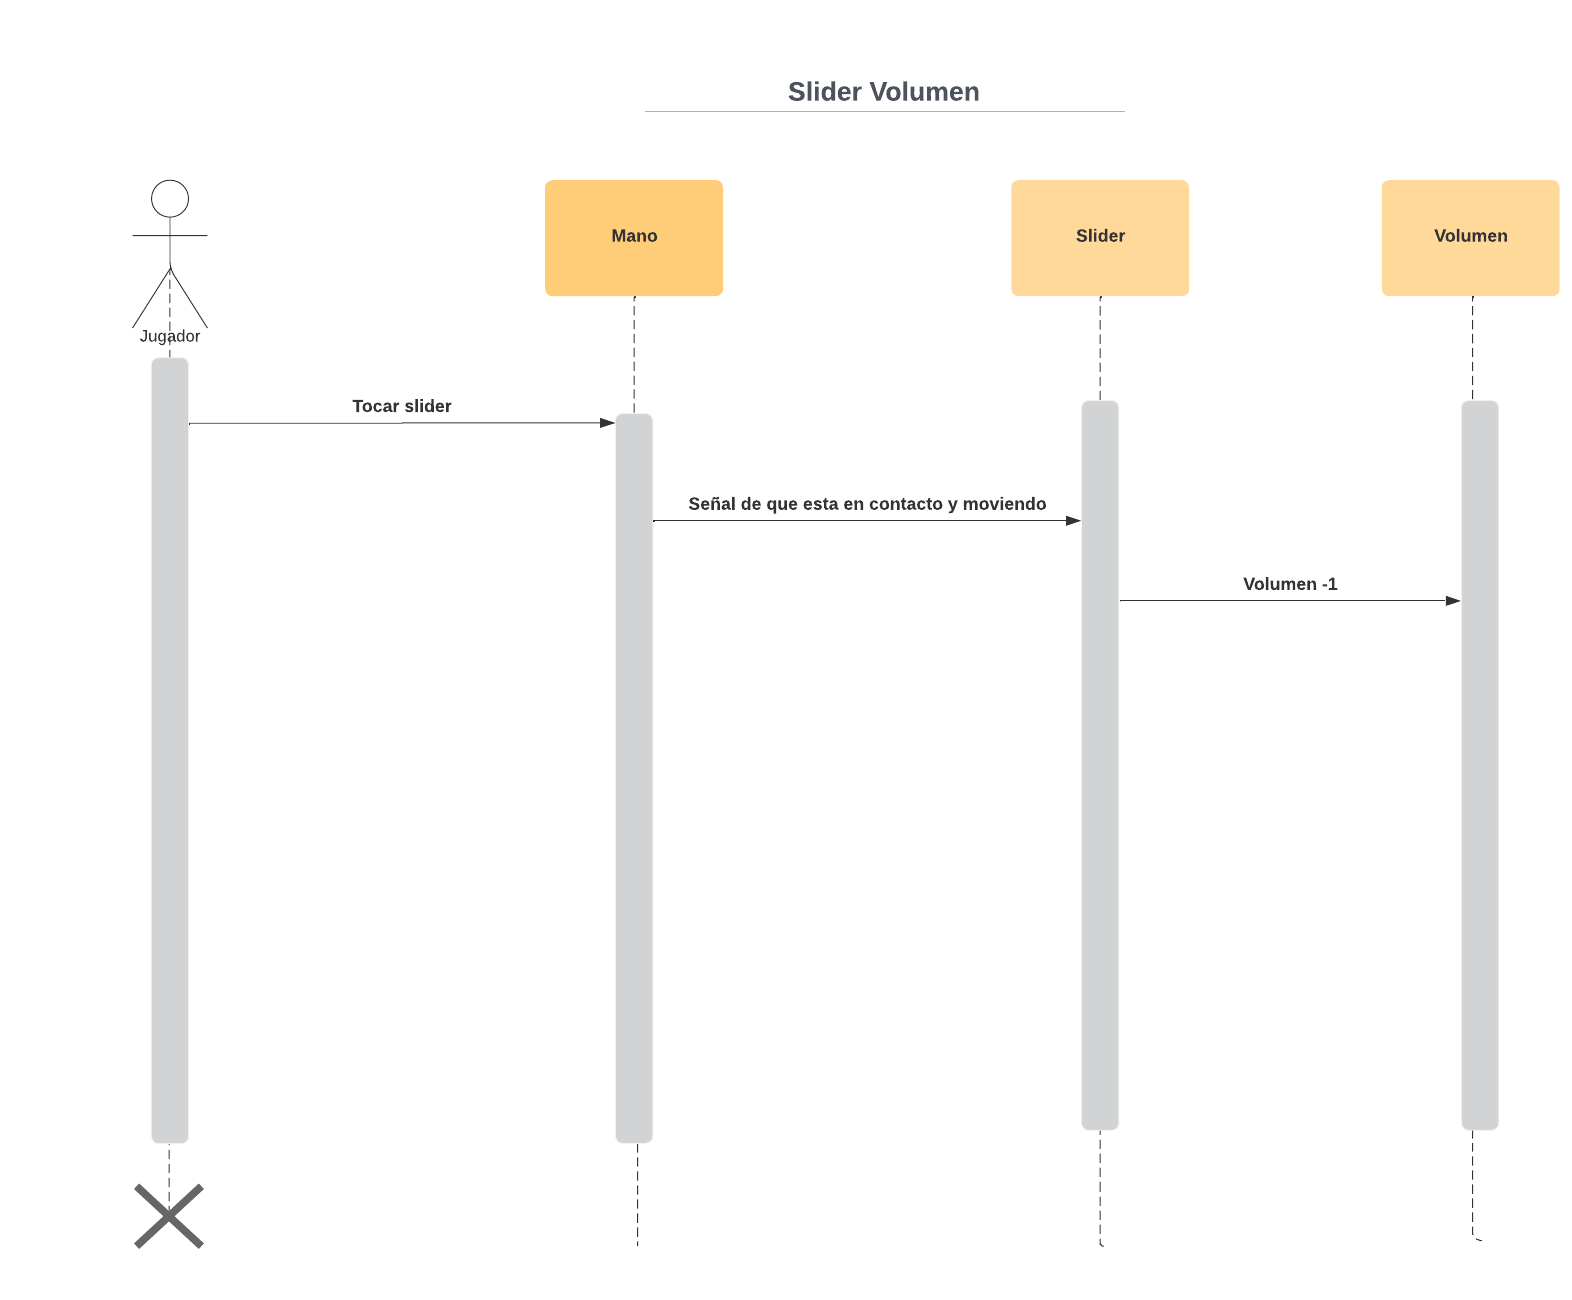
\includegraphics[width=\linewidth]{Diagrama secuencia volumen.png}
  \caption{Diagrama secuencia volumen}
\end{figure}

\begin{figure}  [!htb]
  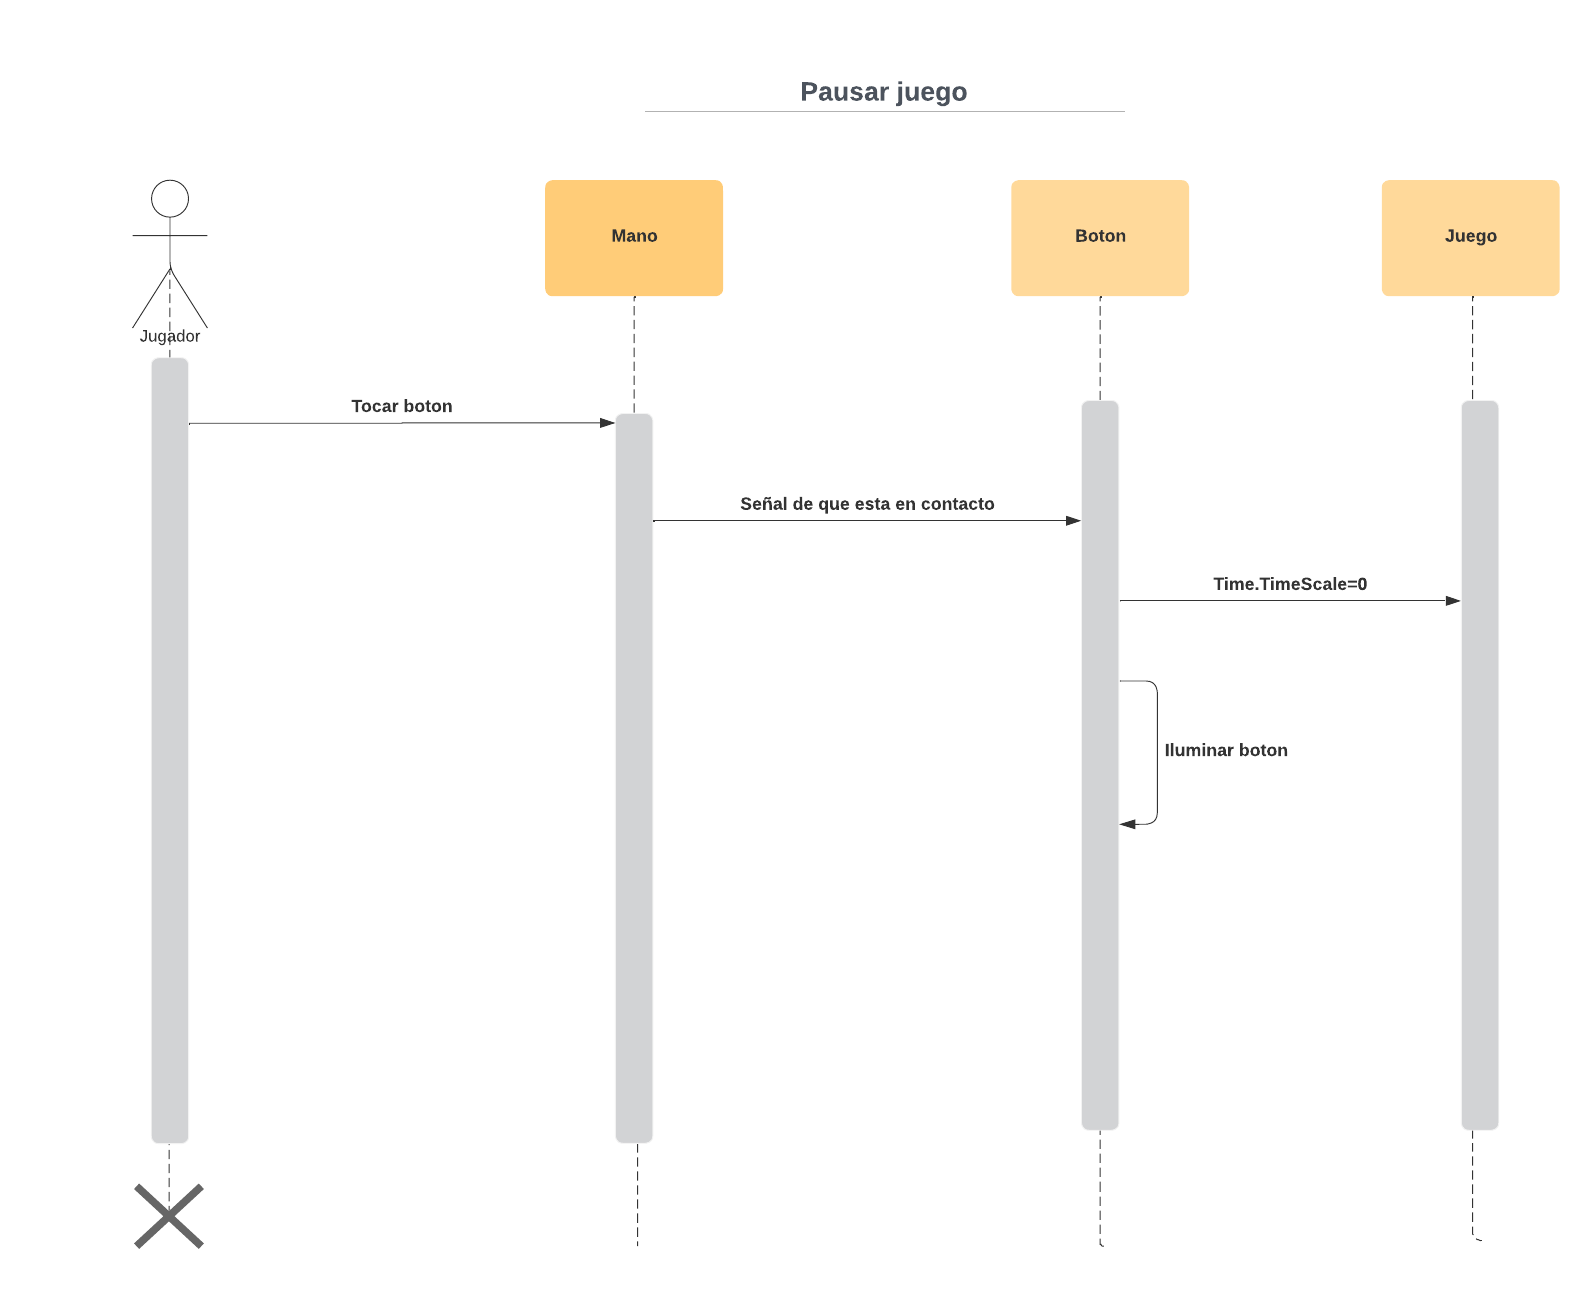
\includegraphics[width=\linewidth]{Diagrama secuencia pausa.png}
  \caption{Diagrama secuencia pausa}
\end{figure}

\begin{figure}  [!htb]
  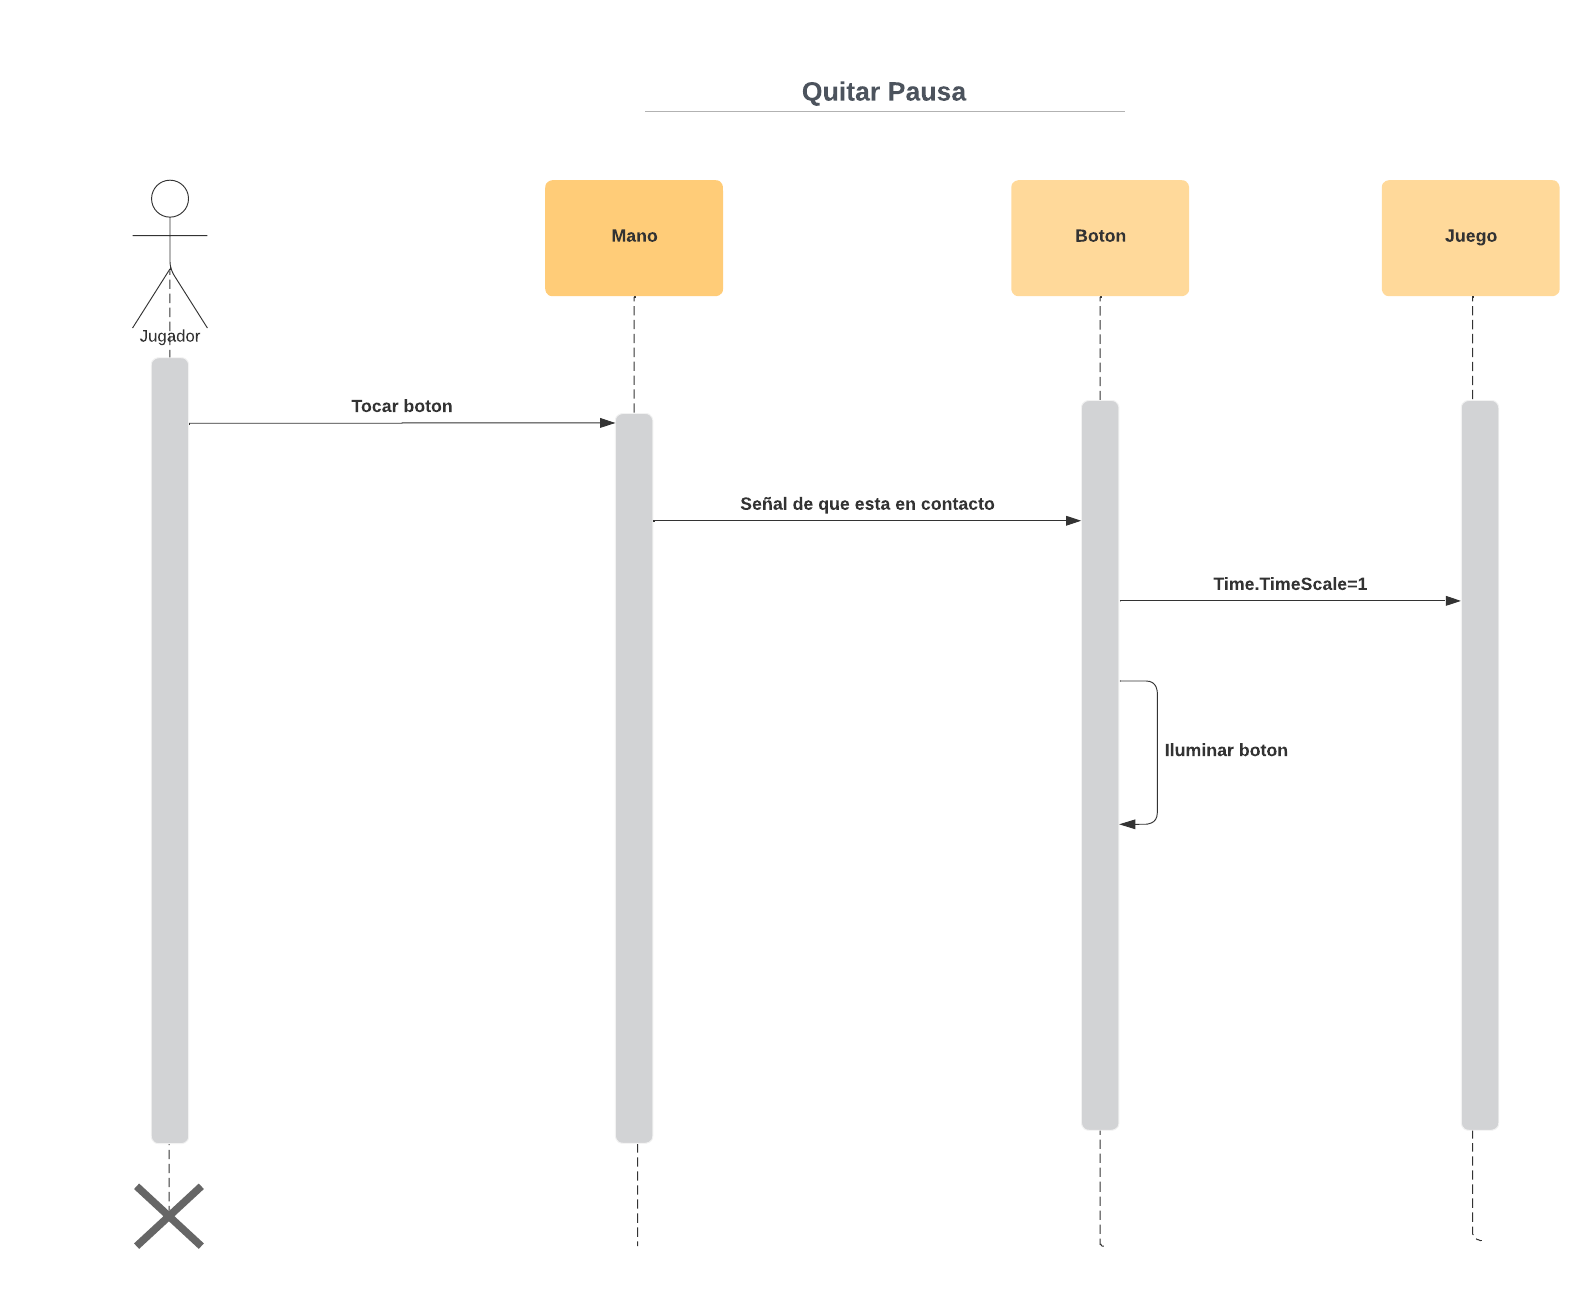
\includegraphics[width=\linewidth]{Diagrama secuencia play.png}
  \caption{Diagrama secuencia quitar pausa}
\end{figure}
\FloatBarrier


\subsection{Diagramas de flujo}
\begin{figure}  [!htb]
  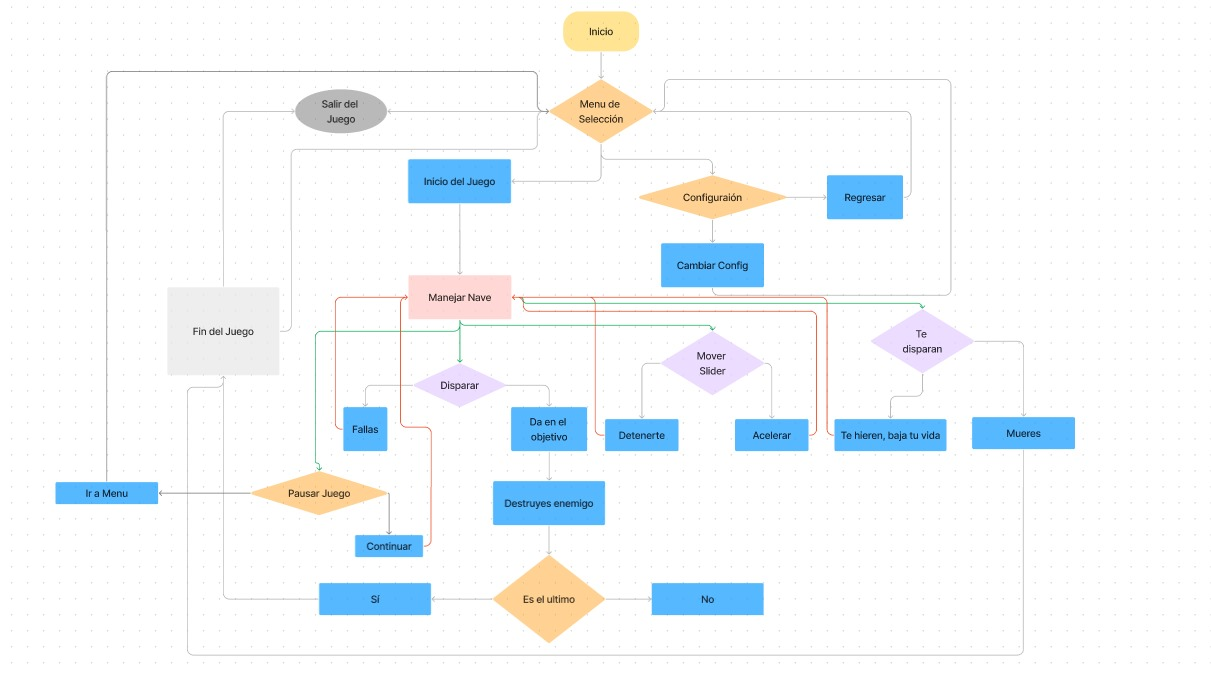
\includegraphics[width=\linewidth]{flujomain.jpg}
  \caption{Diagrama de flujo general}
\end{figure}

\begin{figure}  [!htb]
  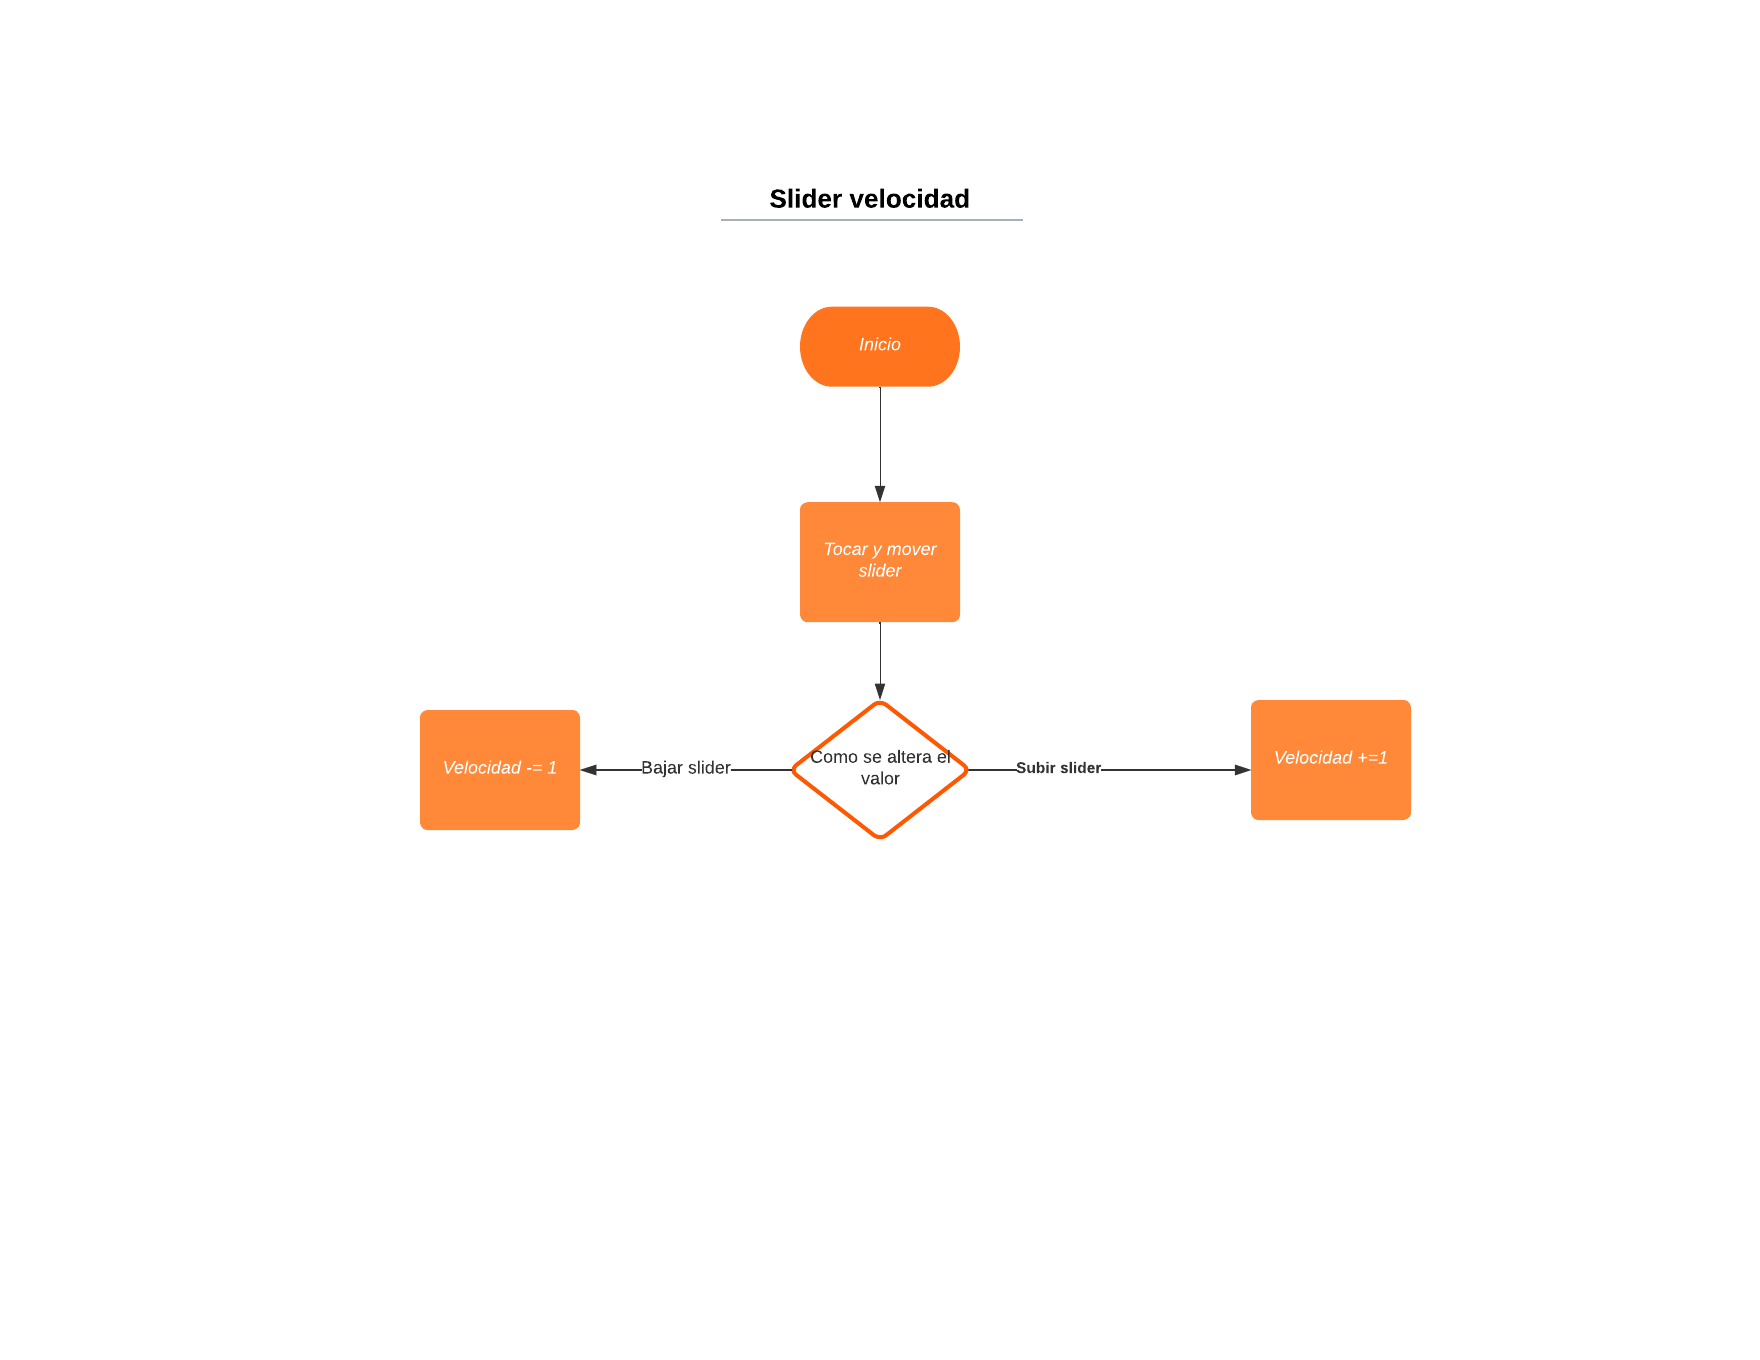
\includegraphics[width=\linewidth]{flujo1.png}
  \caption{Diagrama de flujo slider velocidad}
\end{figure}

\begin{figure}  [!htb]
  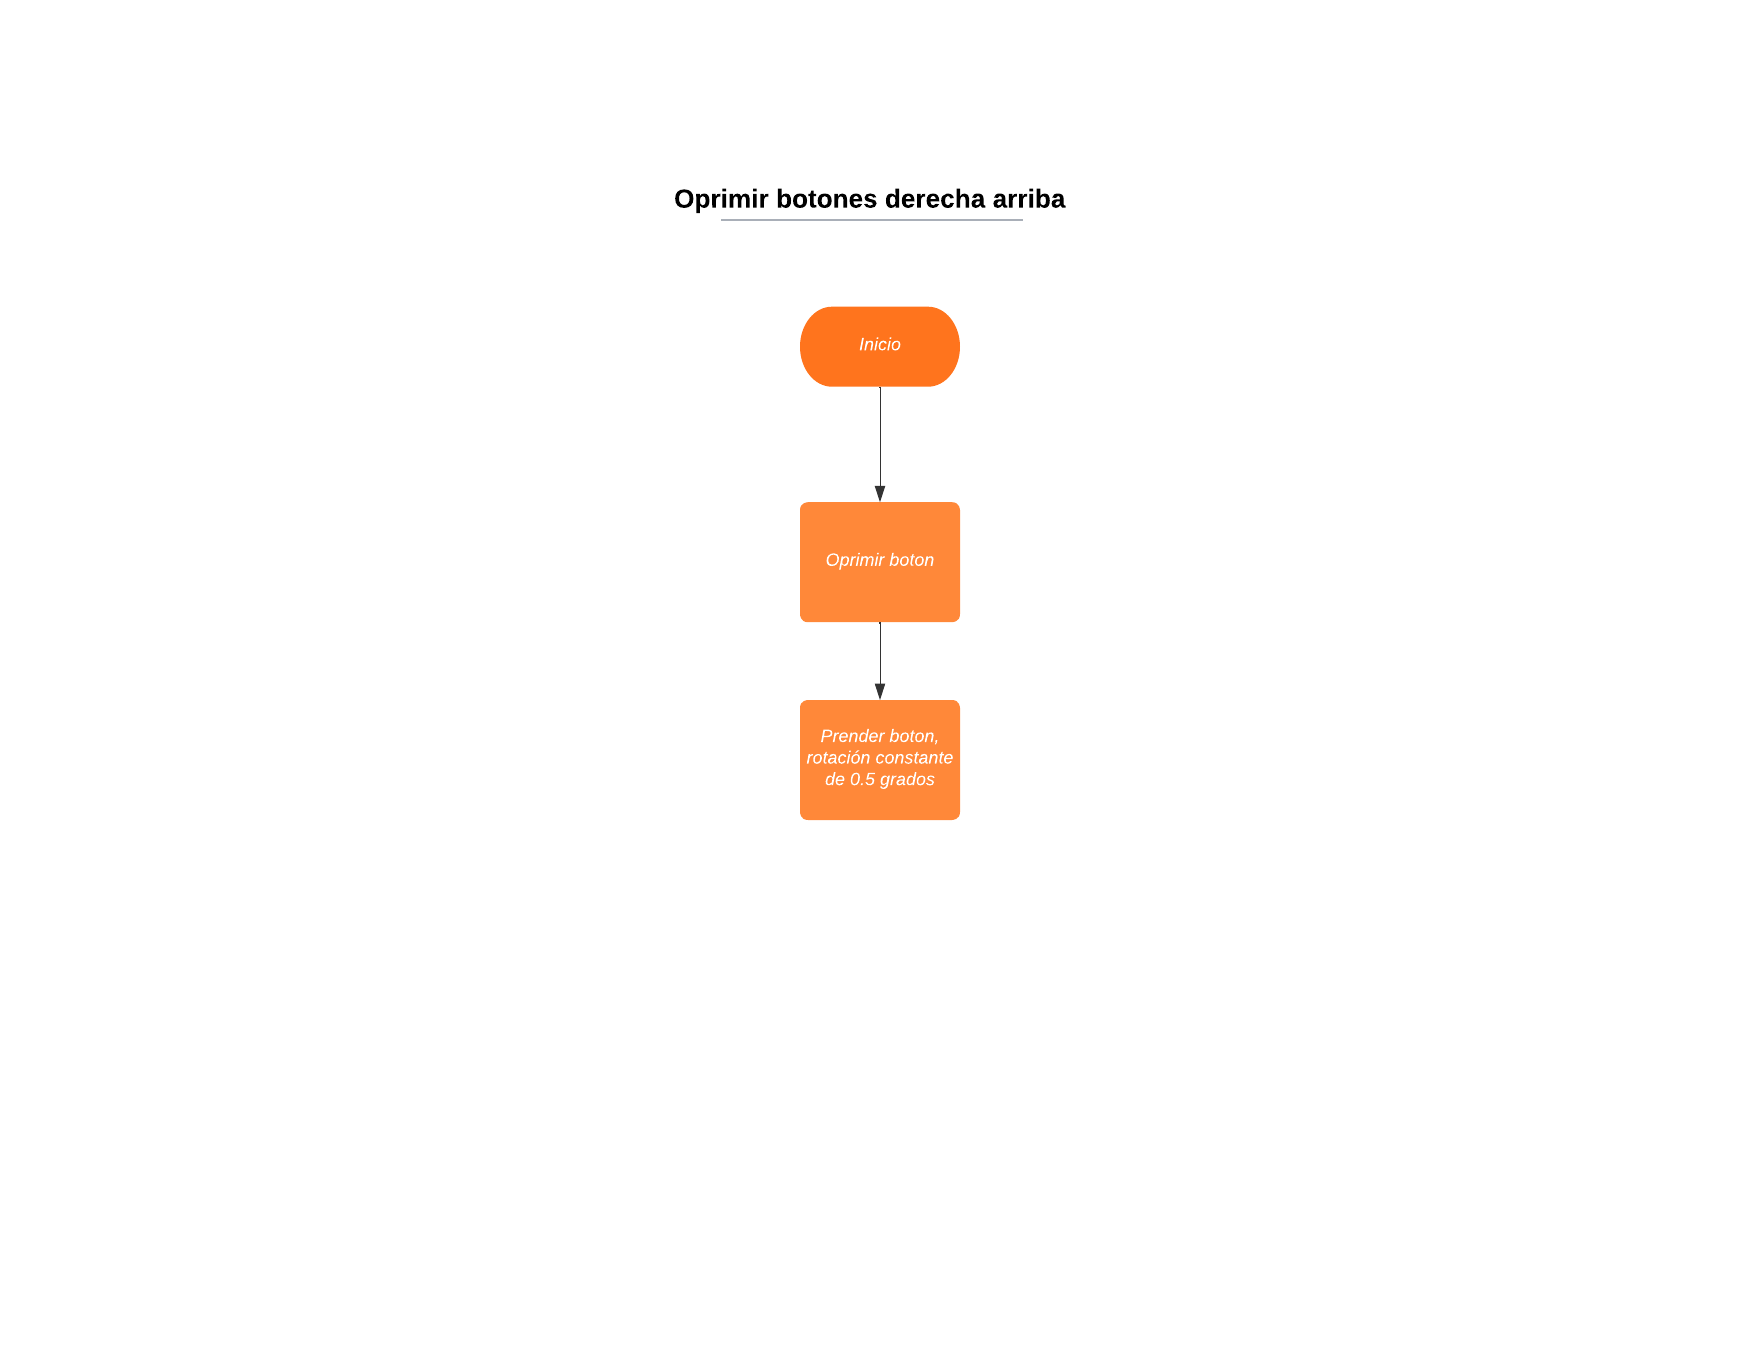
\includegraphics[width=\linewidth]{flujo2.png}
  \caption{Diagrama de flujo botones dirección positiva}
\end{figure}

\begin{figure}  [!htb]
  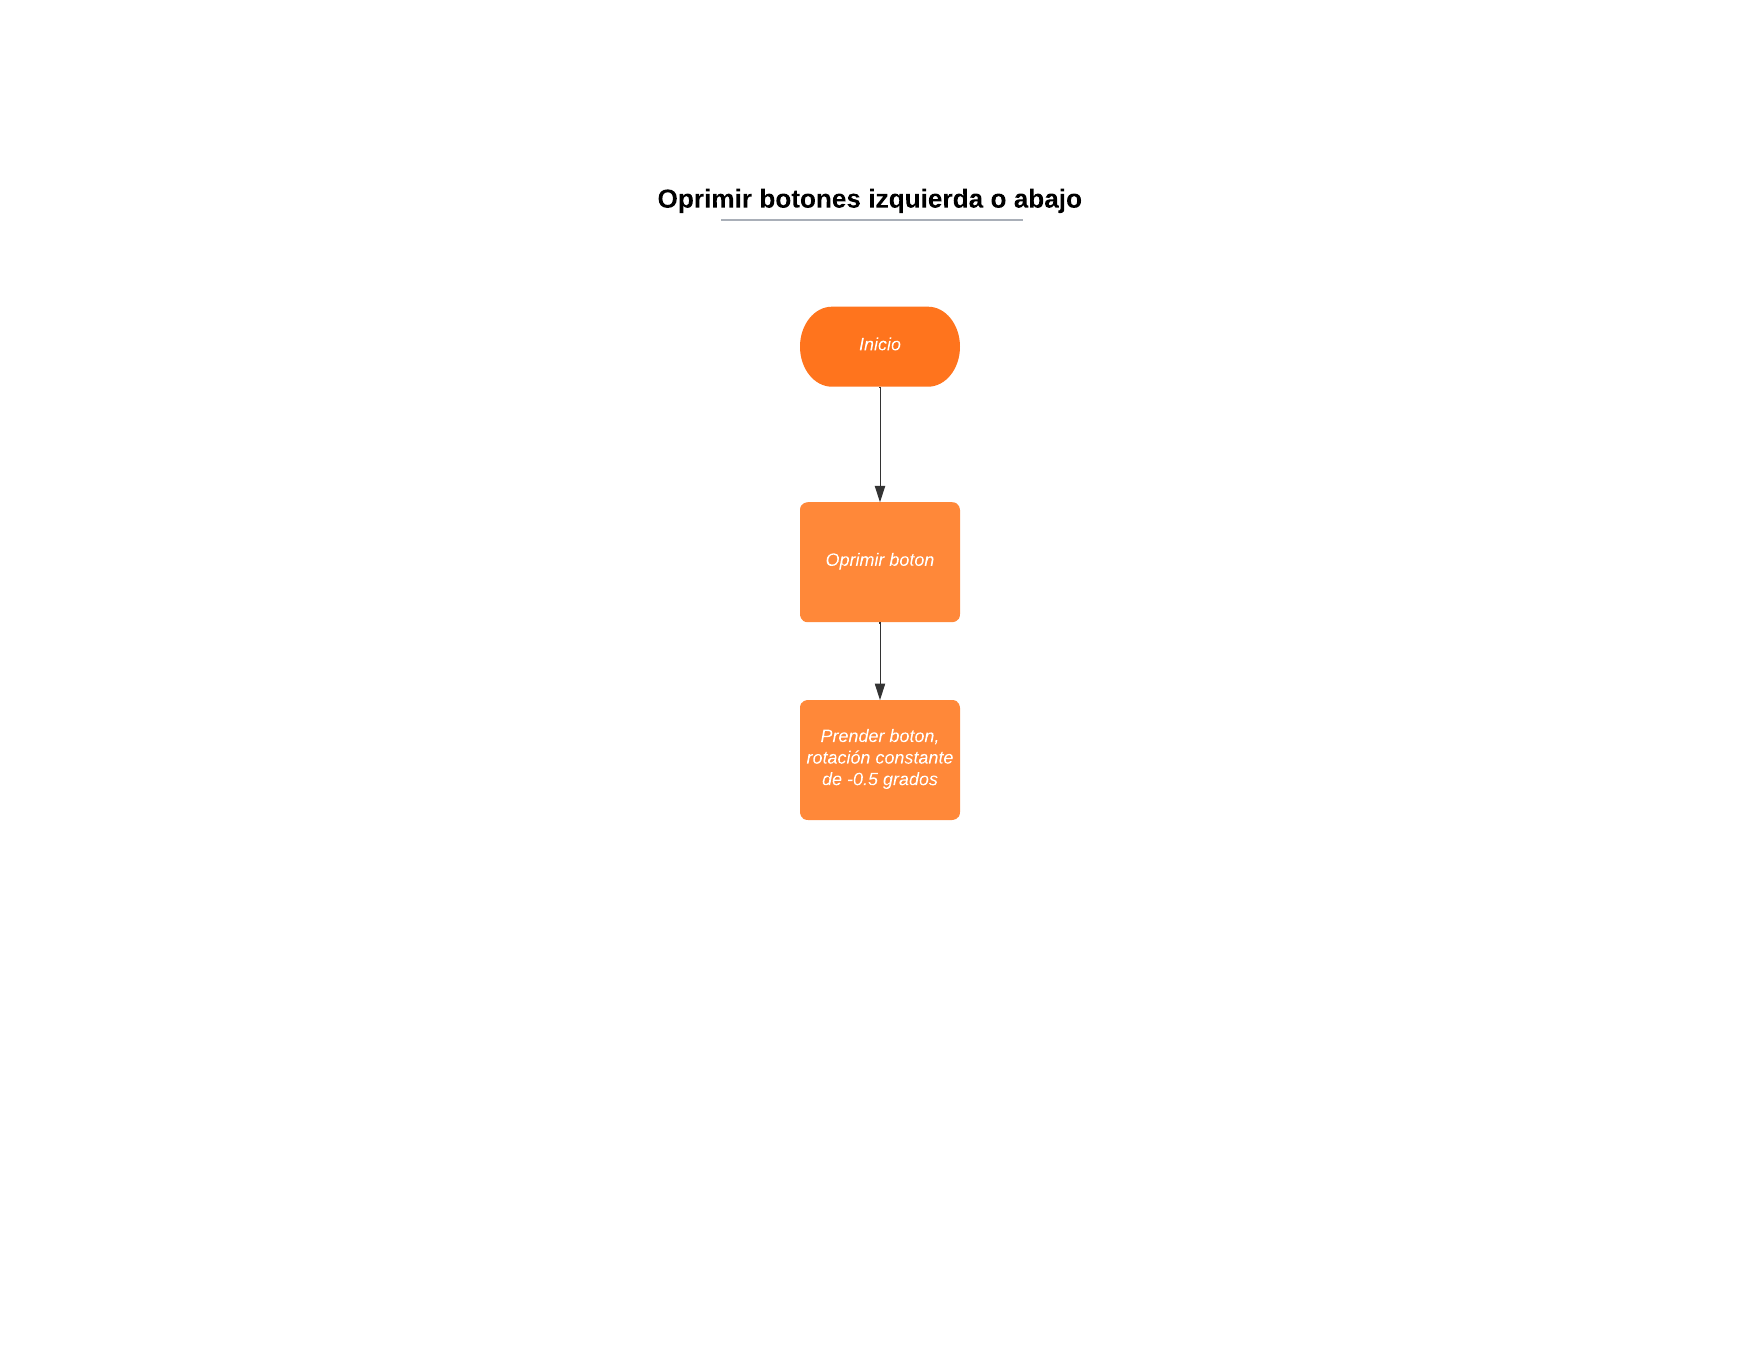
\includegraphics[width=\linewidth]{flujo3.png}
  \caption{Diagrama de flujo botones dirección negativa}
\end{figure}

\begin{figure}  [!htb]
  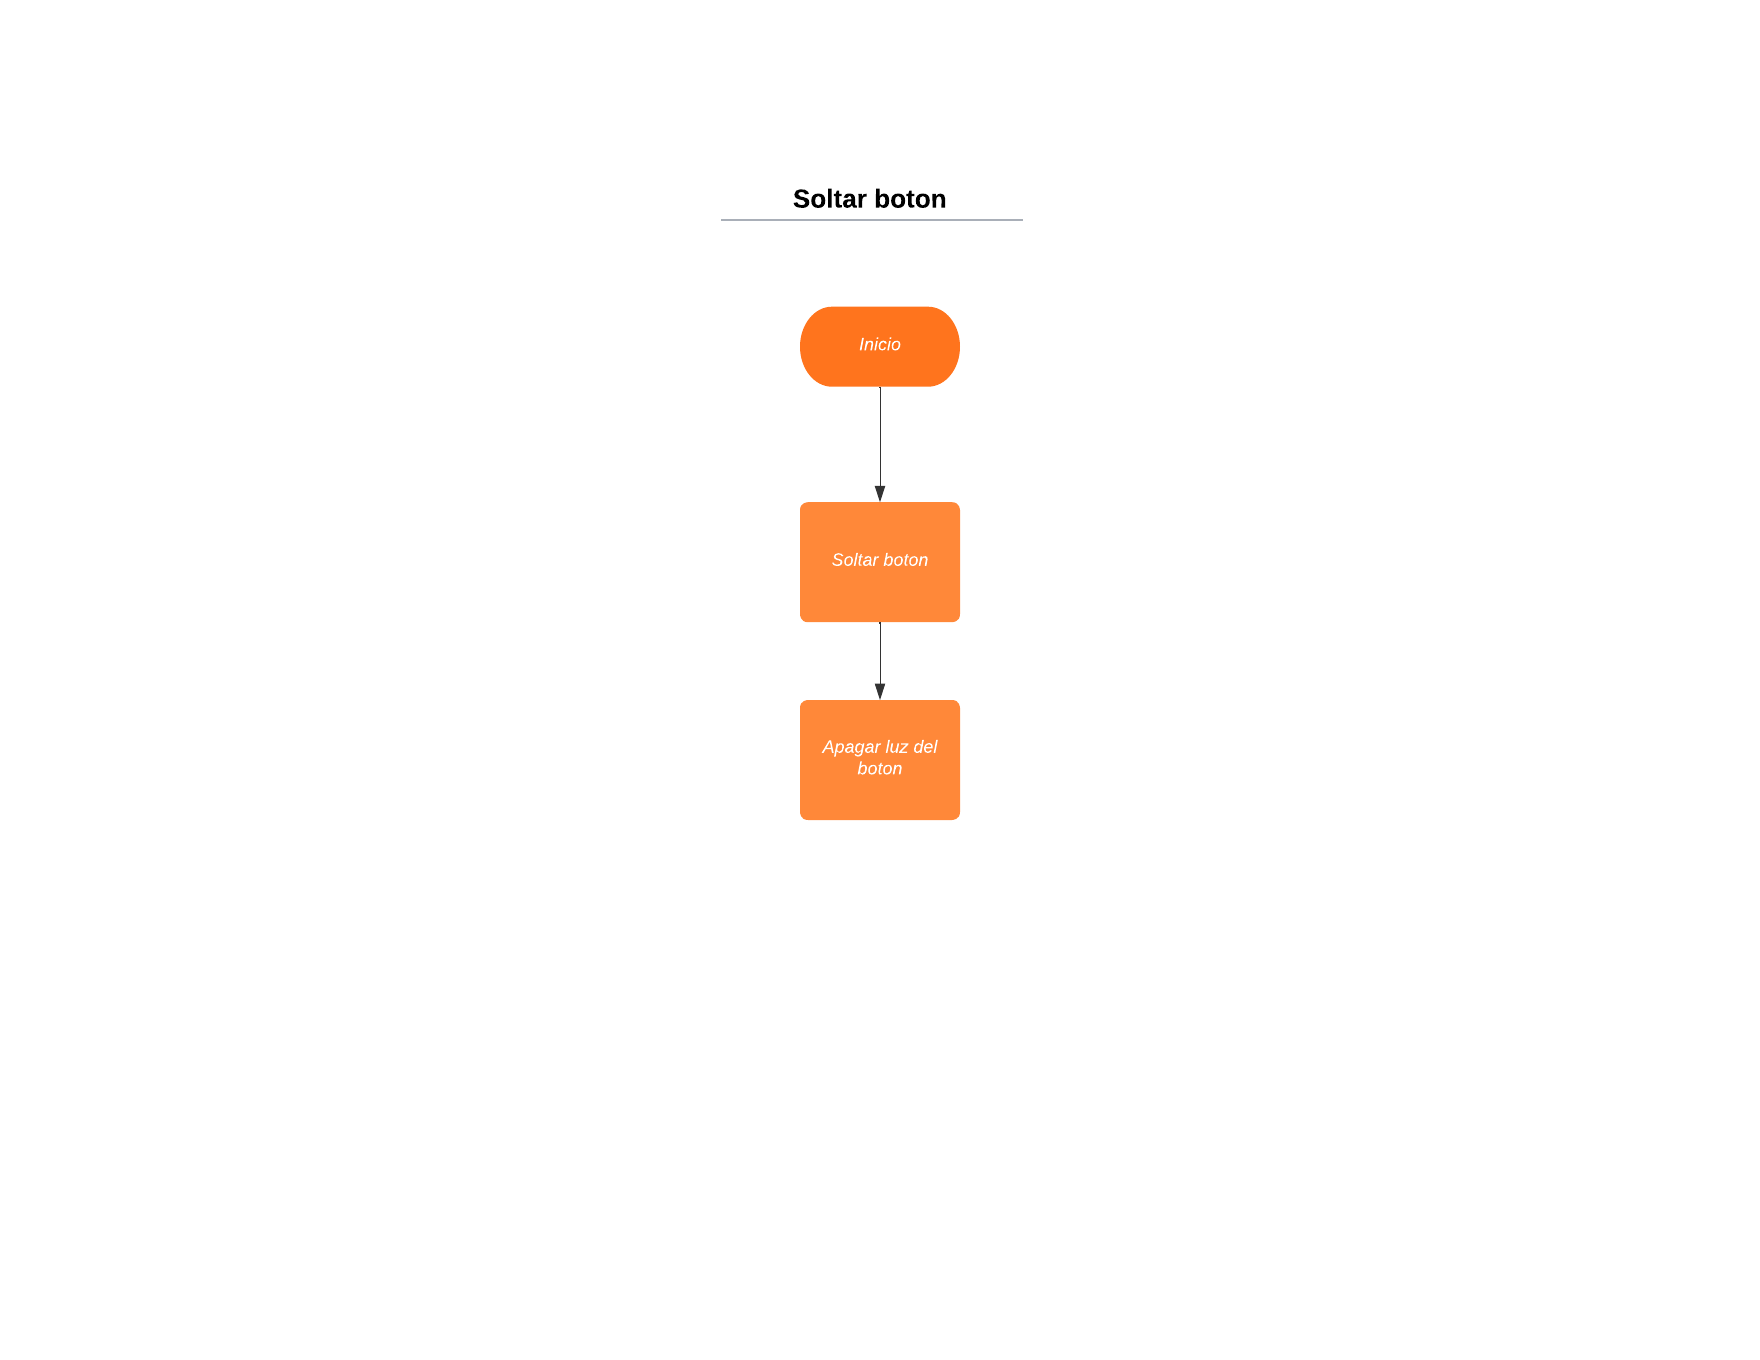
\includegraphics[width=\linewidth]{flujo4.png}
  \caption{Diagrama de flujo soltar boton}
\end{figure}

\begin{figure}  [!htb]
  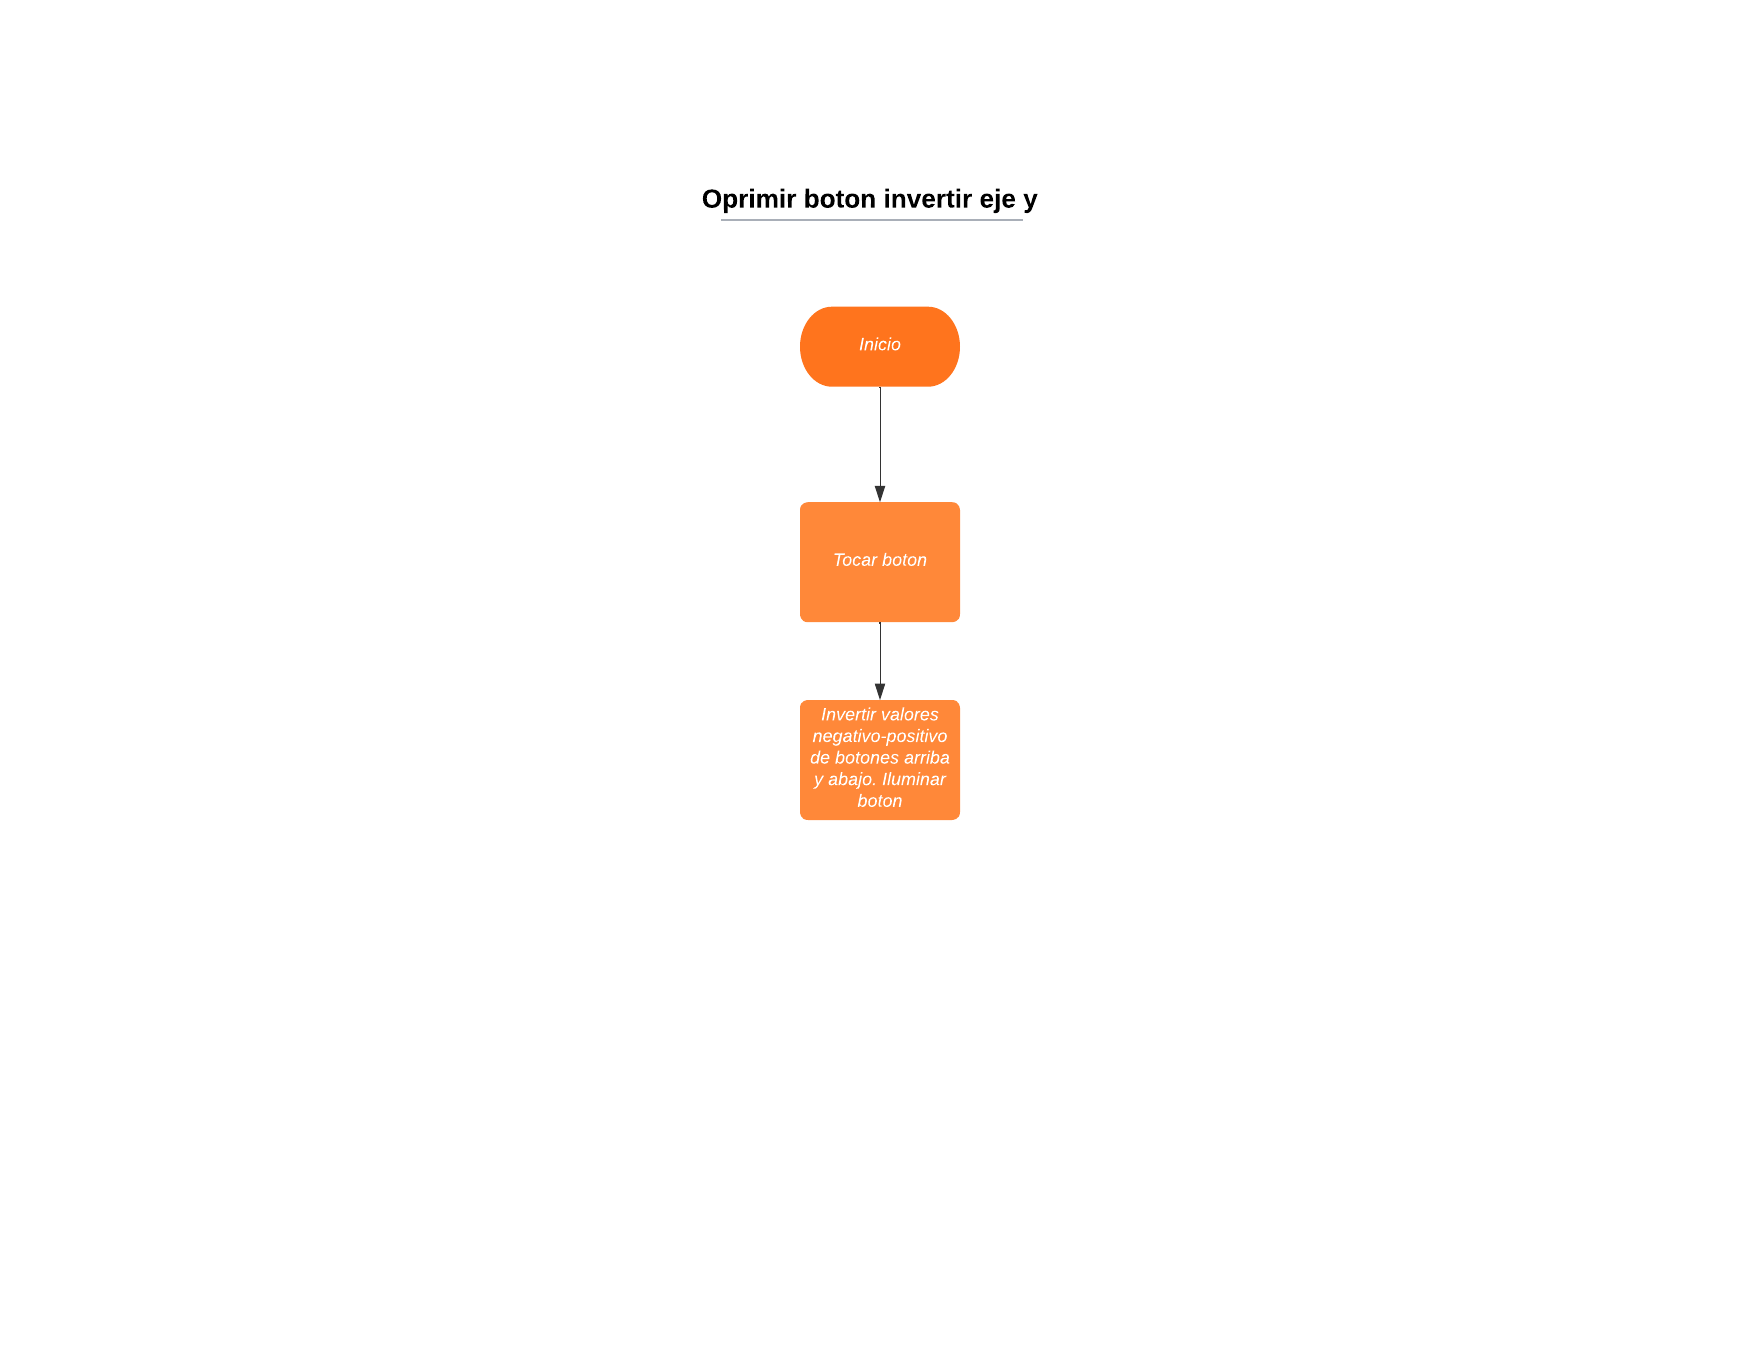
\includegraphics[width=\linewidth]{flujo5.png}
  \caption{Diagrama de flujo invertir eje y}
\end{figure}

\begin{figure}  [!htb]
  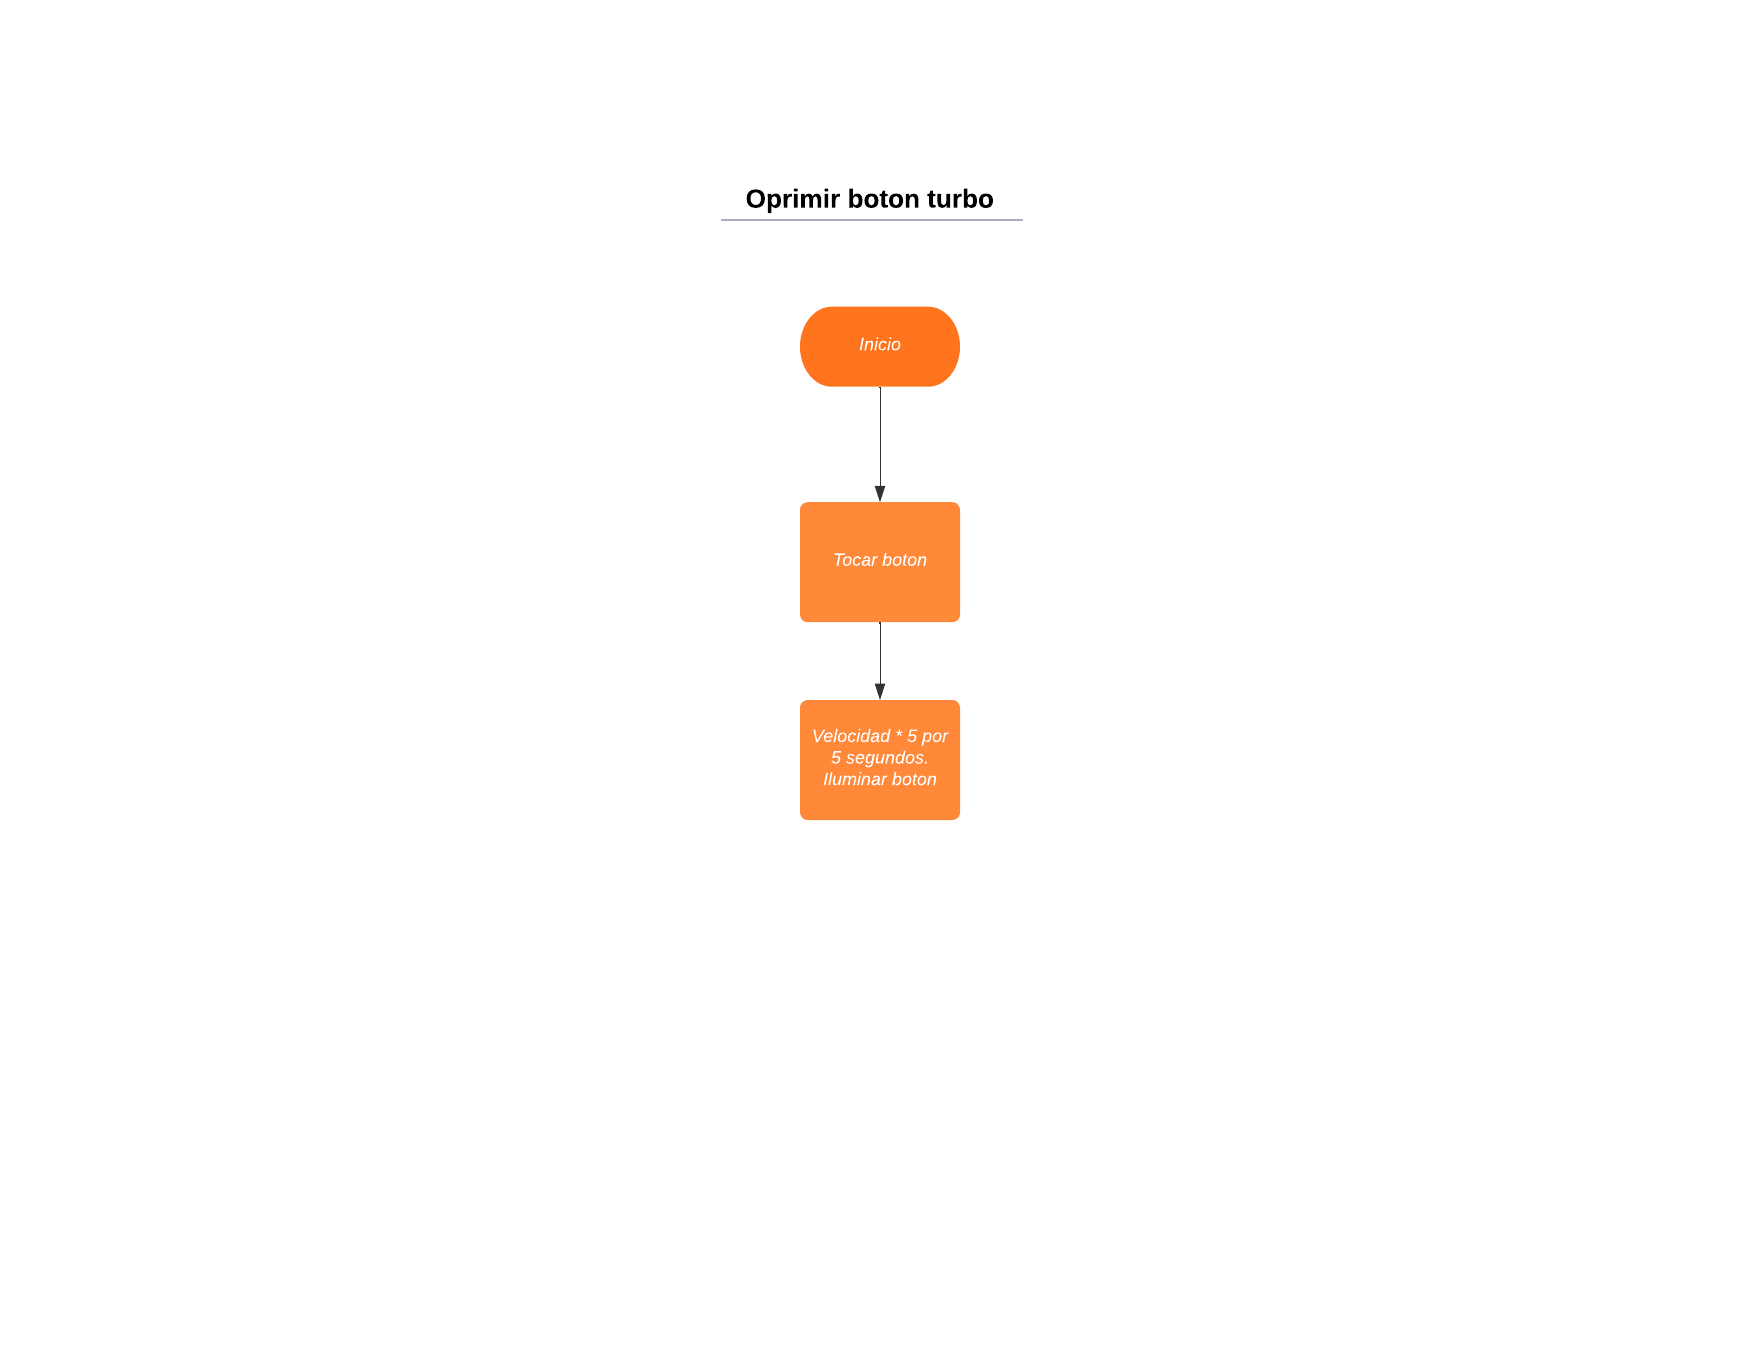
\includegraphics[width=\linewidth]{flujo6.png}
  \caption{Diagrama de flujo turbo}
\end{figure}

\begin{figure}  [!htb]
  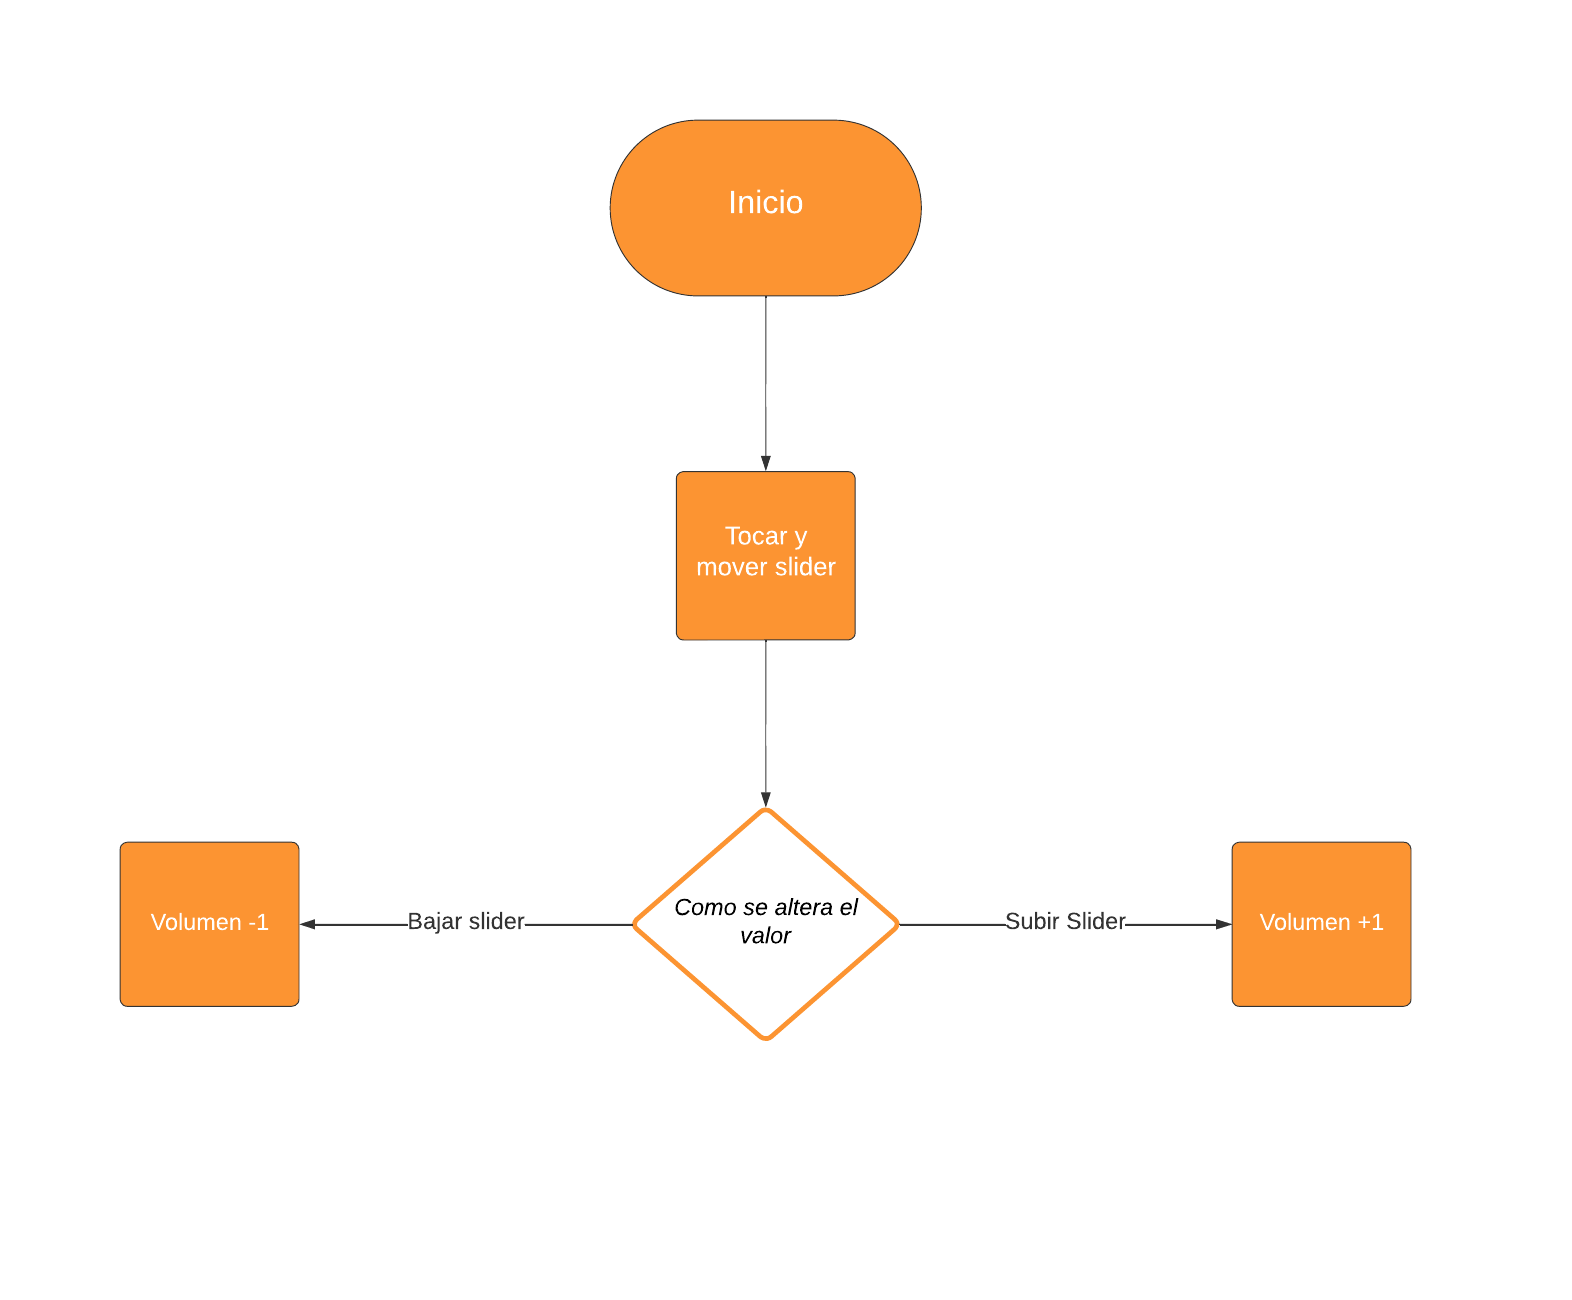
\includegraphics[width=\linewidth]{flujo8.png}
  \caption{Diagrama de flujo volumen}
\end{figure}

\begin{figure}  [!htb]
  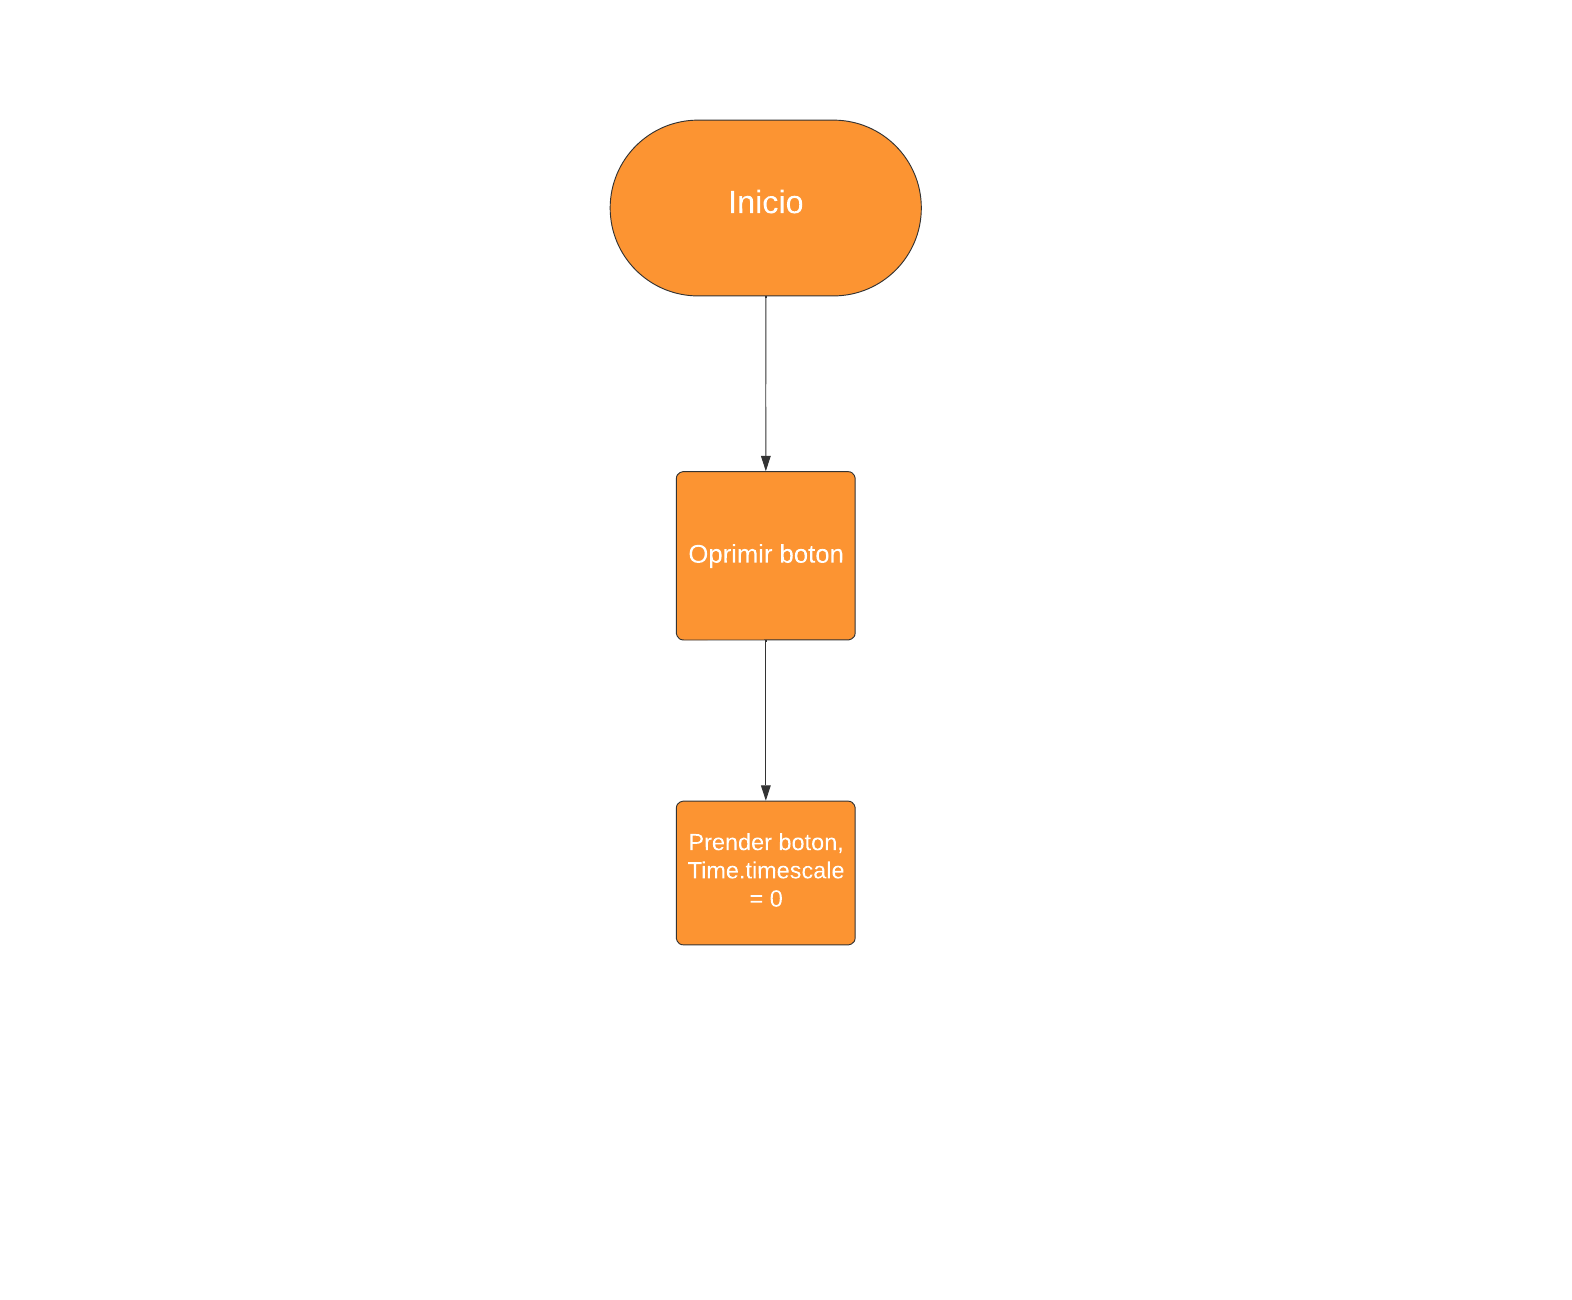
\includegraphics[width=\linewidth]{flujo9.png}
  \caption{Diagrama de flujo pausa}
\end{figure}

\begin{figure}  [!htb]
  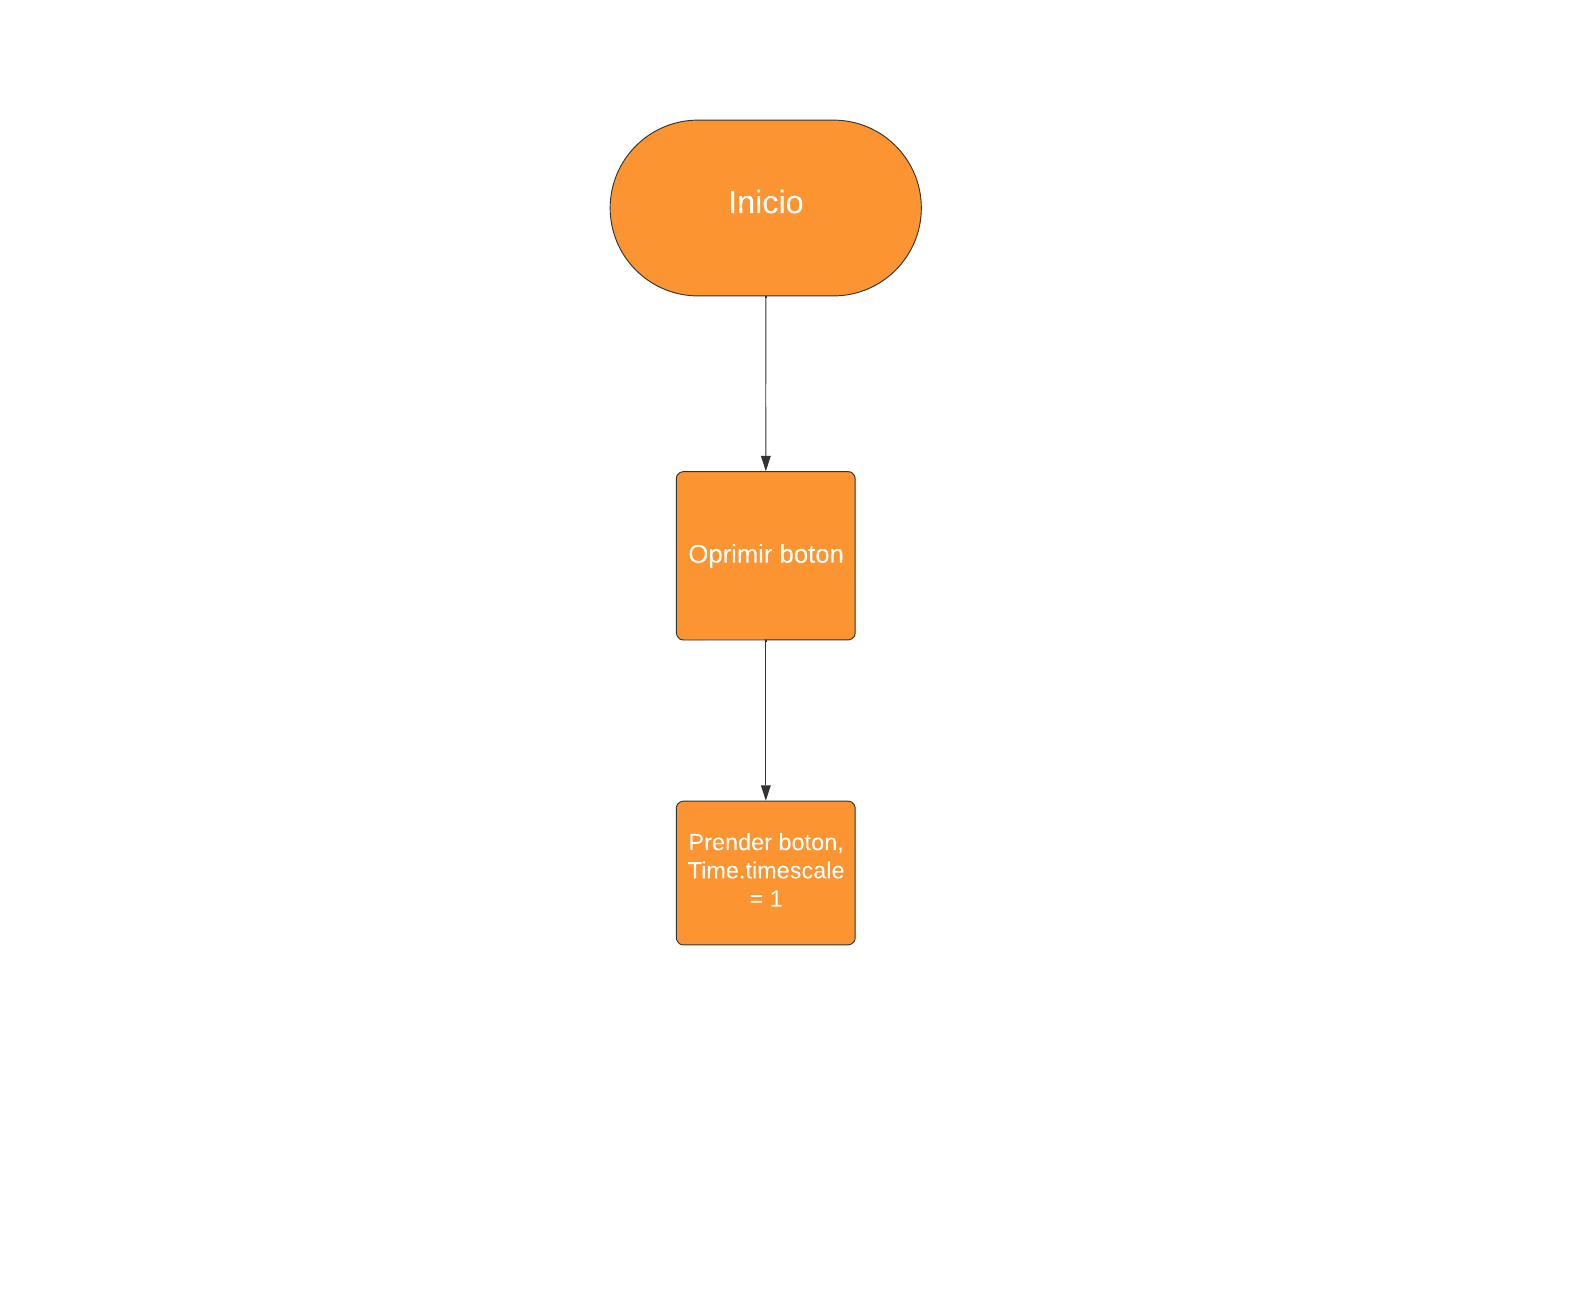
\includegraphics[width=\linewidth]{flujo10.png}
  \caption{Diagrama de flujo quitar pausa}
\end{figure}
\FloatBarrier

\subsection{Diagrama}
\begin{figure}  [!htb]
  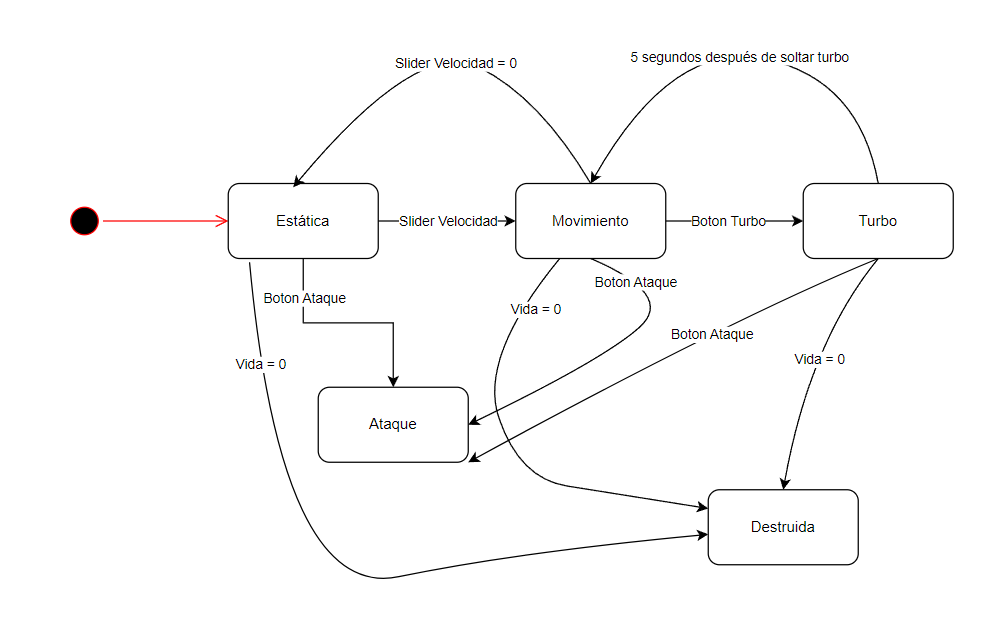
\includegraphics[width=\linewidth]{DiagramaEstados.png}
  \caption{Diagrama de Estados}
\end{figure}
\newpage

\section{Propuesta de Pantallas}\label{pantallas}
\begin{figure} [!htb]
  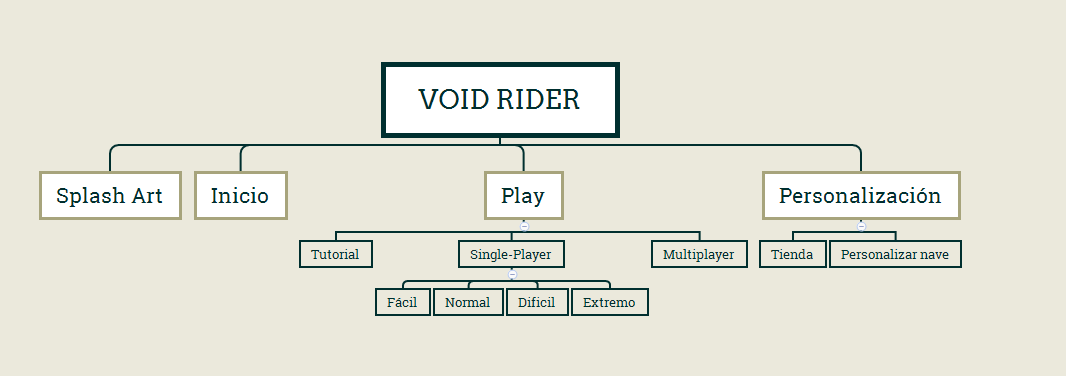
\includegraphics[width=\linewidth]{PantallasVoid.png}
  \caption{Propuesta de pantallas para la aplicación}
\end{figure}

\section{Identidad}\label{identidad}
\subsection{Marca}
\par \textbf{Nombre de la marca:}  ProgramensoStudios
\newpage
\par \textbf{Logo de la marca:}
\begin{figure} [!htb]
  
\includegraphics[width=\linewidth]{progralogo.png}
  \caption{Propuesta para logo de marca}
\end{figure}
\FloatBarrier
\newpage
\subsection{Logo aplicación}
\begin{figure} [!htb]
  
\includegraphics[width=\linewidth]{voidlogo.png}
  \caption{Propuesta para logo de aplicación}
\end{figure}
\FloatBarrier
\subsection{Paleta de color}
\par Los colores usados son los siguientes:
\begin{figure} [!htb]
  
\includegraphics[width=\linewidth]{palette.png}
  \caption{Propuesta para paleta de color}
\end{figure}
\FloatBarrier
\subsection{Tipografía}
\par La tipografía a usar sera \textbf{Roboto} 

\section{Prototipo en Figma}\label{figma}
\par Para ver el prototipo de pantallas en Figma haga \href{https://www.figma.com/file/WSzbb8WSXLqrlPCmQUs2At/Void?type=design&node-id=0%3A1&mode=design&t=Xqxd5z7mG3mFrhSw-1}{Haga click aqui}

\end{document}